\chapter{Saddle Vertex Graph (SVG): A Novel Solution to the Discrete Geodesic Problem}


\section{Overview}\label{sec:svg-overview}

This chapter presents the Saddle Vertex Graph (SVG), a novel solution
to the discrete geodesic problem. The SVG is a sparse undirected
graph that encodes complete geodesic distance information - for
example a geodesic path on the mesh is equivalent to a shortest path
on SVG - which can be solved efficiently using the shortest path
algorithm (e.g., Dijkstra algorithm). The SVG method solves the
discrete geodesic problem from a local perspective. We have observed
that the polyhedral surface has some interesting and unique
properties, such as the fact that the discrete geodesic exhibits a
strong local structure, which is not available on the smooth
surfaces. The richer the details and complicated geometry of the
mesh, the stronger such local structure will be. Taking advantage of
the local nature, the SVG algorithm breaks down the discrete
geodesic problem into significantly smaller sub-problems, and
elegantly enables information reuse. It does not require any
numerical solver, and is numerically stable and insensitive to the
mesh resolution and tessellation. Users can intuitively specify a
model-independent parameter $K$, which effectively balances the SVG
complexity and the accuracy of the computed geodesic distance. More
importantly, the computed distance is guaranteed to be a metric. The
experimental results on real-world models demonstrate significant
improvement to the existing approximate geodesic methods in terms of
both performance and accuracy.


\section{Introduction}
\label{sec:svg-intro}

\begin{figure}[htbp]
\centering
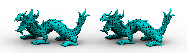
\includegraphics[width=0.95\textwidth]{figs/svg/teaser_2000_final_v2.png}\\
\makebox[3.2in]{Exact polyhedral distance: ICH $127$s; MMP $144$s} \makebox[3.2in]{Our result: $1.96$s, max err. $0.11\%$, rms err. $0.05\%$, mean err. $0.04\%$}\\
\label{fig:teaser}
\caption{It takes $39.1$ seconds to construct an
approximate SVG for the $1.5$M-face Dragon on an Nvidia Tesla K20
GPU. Then any subsequent computation of the single source geodesic
distance takes less than $2.0$s on a $2.66$GHz Intel Xeon machine
using a single core. Therefore, our method is highly desirable to
the applications that require frequent geodesic computations.
Moreover, our method guarantees the computed geodesic distance is a
metric, which distinguishes itself from all the other approximate
geodesic algorithms.}
\end{figure}

The discrete geodesic problem has attracted a great deal of
attention since Mitchell, Mount and Papadimitriou published their
seminal paper in 1987. The MMP algorithm~\cite{Mitchell_Etc:1987}
computes the single-source geodesic distance in $O(n^2\log n)$ time,
where $n$ is the number of vertices of the input mesh. In 1990, Chen
and Han~\cite{Chen_Han:1990} improved the time complexity to
$O(n^2)$, which remains the best-known complexity. However,
extensive experiments have shown that the CH algorithm often runs
$10^3$ to $10^4$ times slower than the MMP algorithm. Xin and Wang
realized that such slowness is due to the extremely large number of
operations to the useless windows (a data structure to that will be
explained later), so they modified the CH algorithm by adopting
window filtering and maintaining windows in a priority queue.
Although the improved CH (or ICH) algorithm has $O(n^2\log n)$ time
complexity, it outperforms both the MMP and the CH algorithms.

So why can the theoretical time complexity not indicate the real
performance in the discrete geodesic problem? The exact geodesic
algorithms, such as MMP, CH and ICH, all adopt the same
computational framework: each edge is partitioned into a set of
intervals, called windows, and each window encodes the geodesic
distance from the source to any point in the interval. The windows
are maintained in either a sorted data structure (like a priority
queue in the MMP and ICH algorithms) or a hierarchical data
structure (like a tree in the CH algorithm). In each iteration, the
algorithms propagate one window across a triangle by computing the
window's children windows. The algorithms terminate when all windows
have been processed. Thus, window complexity is a key factor to
measure the real performance of the algorithm. Mitchell et
al.~\cite{Mitchell_Etc:1987} and Chen and
Han~\cite{Chen_Han:1990} noted that the number of windows is
$O(n^2)$, which means that none of the the window propagation
algorithms can break the theoretical $O(n^2)$ time barrier. On the
other hand, Surazhsky et al.~\cite{Surazhsky_Etc:2005} observed
that the window complexity grows as approximately $O(n^{1.5})$ on
real-world models. In practice, the MMP and the ICH algorithms run
in sub-quadratic time. Surazhsky et
al.~\cite{Surazhsky_Etc:2005} also observed that given a smooth
surface, adding a random noise at each vertex can
 reduce the window complexity significantly. This interesting observation is
confirmed by the experience that computing the geodesic on a bumpy
real-world model usually takes less time than that for a smooth
synthetic model of similar complexity. However, the existing
literature has not addressed the question of the relation between
the algorithm's time complexity and the surface's geometric
features.

All of the existing algorithms compute the globally shortest
geodesic by propagating the distance information in the wavefront
order, thereby tackling the discrete geodesic problem in a global
manner. In this paper, we take a completely different approach,
observing the discrete geodesic's very strong local structure. The
richer the geometric features of the mesh, the stronger such local
structures are. This allows us to break down the original problem
into easily solvable sub-problems.

In moving towards this goal, we propose the \textit{Saddle Vertex
Graph (or SVG)}, a novel method for computing the geodesic distance
on a triangle mesh. The SVG is a sparse undirected graph that has
the same vertex set as the input mesh. Each SVG edge corresponds to
a direct geodesic path that does not pass through any saddle
vertices. The SVG encodes complete geodesic information in that a
geodesic path on the mesh is a shortest path on the corresponding
SVG; therefore, the discrete geodesic problem is converted into a
shortest path problem.

The SVG has several unique features that distinguish it from other
algorithms.
\begin{itemize}
% the unified framework
%\item Firstly, the SVG elegantly enables information reuses, which provides a unified framework to compute all types of discrete
%geodesics, including geodesic path, single-source, multiple-sources,
%and all-pairs geodesic.

\item Firstly, it is highly efficient, since computing the single-source geodesic distances on a real-world model takes $O(Dn\log n)$ time,
where $n=|V|$ is the number of mesh vertices and $D$ ($D\ll n$)
measures the complexity of the SVG. Moreover, as the Dijkstra
algorithm does not involve any numerical computation, the SVG is
much faster than the fast marching method (FMM).

\item Secondly, users can intuitively control the accuracy by
specifying the local covering range of the saddle vertices. The
computed geodesic distance is guaranteed to be a metric, i.e.,
satisfying the symmetry condition and the triangle inequality. Since
it does not require any numerical solver, the SVG method is
numerically stable and robust to the mesh triangulation and
tessellation.

% the quality
\item Thirdly, the SVG exhibits a strong local structure that enables it to be constructed in a completely local and parallel manner. Furthermore,
the SVG's average degrees depend on the model's details, and is
insensitive to the mesh size. The more details and complicated
geometry the model has, the stronger such local characteristics are,
and the \textit{smaller} the average degree of the SVG vertices.
Therefore, the results for SVG are much better for real-world models
with details than the poor results that existing approximate
algorithms often produce.

% shortest path
\item Last but not least, it naturally links the discrete
geodesic problem with the shortest path problem, which has been
studied extensively. Therefore, the discrete geodesic problem can
immediately take advantage of existing resources as well as new
developments in the shortest path problem (such as parallelization).
\end{itemize}

\section{Preliminary}
\label{sec:preliminary} Let $M=(V,E,F)$ be a triangle mesh
representing an orientable 2-manifold where $V$, $E$ and $F$ are the
vertex, edge and face sets respectively. Let $n=|V|$ be the number
of vertices. Throughout the paper, we always assume the mesh $M$ is
connected.

The total vertex angle of a vertex $v\in V$ is the sum of interior
angles formed by the edges incident at $v$. A vertex $v$ is called
{\em spherical} if its total vertex angle is less than $2\pi$, {\em
Euclidean} if the total vertex angle equals $2\pi$, and {\em saddle}
if the total vertex angle is greater than $2\pi$. Let $\gamma(p,q)$
denote a geodesic path between $p$ and $q$. Note that there may be
multiple geodesic paths between $p$ and $q$. We denote $d(p,q)$ the
\textit{globally} shortest geodesic distance between $p$ and $q$.


Clearly, a geodesic path must be a straight line inside a triangle.
When crossing over an edge, the geodesic path must also correspond
to a straight line if the two adjacent faces are unfolded into a
common plane. Mitchell et al.~\cite{Mitchell_Etc:1987} proved
the following theorems of
 discrete geodesics.
\begin{itemize}
\item There exists a geodesic path from the source to any other point on the surface.
\item A geodesic path goes through an alternating sequence
of vertices and edges such that the unfolded image of the path along
any edge sequence is a straight line segment and the angle of the
path passing through a vertex is greater than or equal to $\pi$.
\item A geodesic path cannot pass through a
spherical vertex unless it is an endpoint or a boundary point.
%\item When a geodesic path passes a saddle vertex, ...
\end{itemize}

\if 0 Both the MMP and CH algorithms adopt the same computational
framework: each edge is partitioned into a set of intervals, which
are called windows. Each window groups a set of geodesic paths,
which share the same face and edge sequence. Intuitively speaking, a
window that is associated to an interval encodes the exact geodesic
distance from the source to any point in the interval. The windows
are maintained in either a sorted data structure (like a priority
queue in the MMP and ICH algorithms) or a hierarchical data
structure (like a tree in the CH algorithm). In each iteration, the
algorithms propagate one window across a triangle by computing the
window's children windows and performing clipping or merging if
necessary, which can add, modify, or remove existing windows. The
algorithms terminate when all windows have been processed. \fi

Both the MMP and CH algorithms adopt a similar window propagation
framework, in which the saddle vertices play a critical role by
acting as ``relays'' that propagate the windows from the source
towards the destination. As Figure~\ref{fig:saddle}(a) shows, when a
geodesic wavefront passes through a saddle vertex $v$, it splits
into three arcs; the left and right arcs remain centered at the
original source, but the central arc is originated at $v$. These
arcs are then propagated with respect to their own centers, causing
the geodesic path to be split at $v$ (see
Figure~\ref{fig:saddle}(b)). This is the reason that saddle vertices
are called pseudosources in the MMP, CH, and ICH algorithms. As
Figure~\ref{fig:saddle}(c) shows, a typical geodesic path $\gamma$
may pass through one or more saddle vertices, and two different
geodesic paths $\gamma(s_1,t_1)$ and $\gamma(s_2,t_2)$ may share
common segments.

\begin{figure}[htbp]
\centering
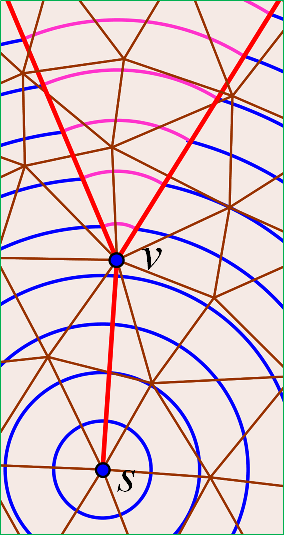
\includegraphics[width=0.3\textwidth]{figs/svg/wavefront_label.png}\hspace{0.05in}
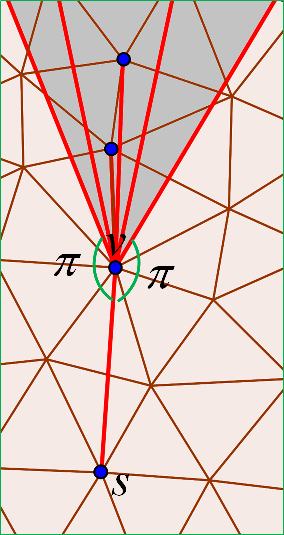
\includegraphics[width=0.3\textwidth]{figs/svg/geodesic_split2.png}\hspace{0.05in}
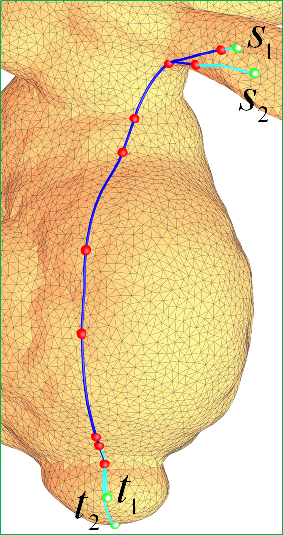
\includegraphics[width=0.3\textwidth]{figs/svg/shared_path_labels2.png}\\
\makebox[0.3\textwidth]{(a)}\makebox[0.3\textwidth]{(b)}\makebox[0.3\textwidth]{(c)}\\
\vspace{-0.1in} \caption{Saddle vertex and geodesic path. (a) A
saddle vertex $v$ has the total vertex angle $\sum \theta_i > 2\pi$.
When passing through $v$, the geodesic wavefront, a circle centered
at the source $s$, splits into three arcs. The middle arc (in pink)
is centered at $v$, and the left and right arcs remain centered at
$s$. (b) The incoming geodesic path $\gamma$ splits at the saddle
vertex $v$. All the outgoing geodesic paths are in the fanned area
(shaded in dark grey), which has angle $\sum \theta_i - 2\pi$. (c) A
long geodesic path $\gamma$ usually passes through one or more
saddle vertices (the red points), which partition $\gamma$ into
several segments. Two geodesic paths $\gamma(s_1,t_1)$ and
$\gamma(s_2,t_2)$ may share a large portion of their paths. }
\label{fig:saddle}
\end{figure}

\vspace{-0.1in} \noindent\textbf{Remark.} A geodesic path
$\gamma(s,t)$ on a smooth surface is both straightest and locally
shortest. Therefore, two geodesic paths cannot share a common
segment. However,  the locally shortest geodesic path is not
equivalent to the straightest geodesic path on a piecewise linear
surface~\cite{Polthier_Schmies:1998}. Due to this fundamental
difference between the smooth surfaces and the polygonal surfaces,
the discrete geodesic has some unique features that are not
available in the smooth counterpart. For example, the shortest
geodesic cannot be extended through a spherical vertex since it
could be shortened by moving off the corner. There exists a family
of extension of a geodesic through a saddle vertex. Two or more
geodesic paths can share common segments with saddle vertices as
endpoints. Taking advantages of these unique features of the
discrete geodesic, we define our saddle vertex graph in the next
section.


\section{Saddle Vertex Graph}
\label{sec:svg}

\subsection{Definition}
\label{subsec:def}

\noindent\textbf{Definition 1.}  Consider $\gamma(p,q)$ a globally
shortest geodesic path between $p$ and $q$. $\gamma$ is called
\textit{direct} if it does not pass through any saddle vertices, and
\textit{indirect} otherwise.

An indirect path contains one or more saddle vertices, by which the
geodesic path is partitioned into several segments, each of which is
a direct path.

Let $V_S$ denote the set of saddle vertices and $V_N$ denote the set
of non-saddle vertices (i.e., Euclidean and spherical vertices),
then we have $|V|=|V_S|+|V_N|$.

\noindent\textbf{Definition 2.} Consider a non-saddle vertex $v\in
V_N$. The \textit{saddle neighbors} of $v$, denoted by
$\mathcal{S}(v)$, are the saddle vertices which can be reached from
$v$ via a direct geodesic path. Similarly, the \textit{non-saddle
neighbors} of $v$, denoted by $\mathcal{N}(v)$, are the non-saddle
vertices which can be reached from $v$ via direct geodesic paths.

\noindent\textbf{Definition 3.} The \textit{direct neighbors} of a
vertex $v\in V$ are the vertices that can be reached from $v$
via direct geodesic paths.

\noindent\textbf{Definition 4.} An S-S edge is a \textit{direct}
geodesic path between two saddle vertices. An N-S edge is a
\textit{direct} geodesic path between a non-saddle vertex and a
saddle vertex. An N-N edge is a \textit{direct} geodesic path
between two non-saddle vertices. Let $E_{SS}$, $E_{NS}$, and
$E_{NN}$ denote the set of S-S edges, N-S edges, and N-N edges
respectively,
\begin{eqnarray}
\nonumber & &E_{SS}=\{\gamma(p,q)|p,q\in
V_S~\mathrm{and}~\gamma(p,q)~\mathrm{is~direct}\},\\
\nonumber & &E_{NS}=\{\gamma(p,q)|p\in V_N, ~q\in
V_S~\mathrm{and}~\gamma(p,q)~\mathrm{is~direct}\}, \\
\nonumber & &E_{NN}=\{\gamma(p,q)|p,q\in
V_N~\mathrm{and}~\gamma(p,q)~\mathrm{is~direct}\}.
\end{eqnarray}
Clearly, the sets $E_{SS}$, $E_{NS}$ and $E_{NN}$ are disjoint.
Figure~\ref{fig:svg} shows examples of S-S, N-S and N-N edges on the
Bimba model. We are now ready to define the Saddle Vertex Graph.

\noindent\textbf{Definition 5.} The SVG associated to a triangle
mesh $M=(V,E,F)$ is an undirected graph $S=S_1\bigcup S_2\bigcup
S_3$ formed in three tiers.
\begin{itemize}
\item  The tier 1 sub-graph $S_1=(V_S, E_{SS})$, which is the core network, consists of all
the S-S edges connecting the saddle vertices via direct geodesic
paths.
\item The tier 2 sub-graph $S_2=(V_S\bigcup V_N, E_{NS})$ contains the N-S edges, which are
the direct geodesic paths connecting the non-saddle vertices to the
saddle vertices.
\item The tier 3 sub-graph $S_3=(V_N,E_{NN})$ contains the N-N edges, which are the
direct geodesic paths connecting the non-saddle vertices.
\end{itemize}

The SVG is connected and encodes the complete geodesic paths between
any two vertices.

\noindent\textbf{Proposition 1.}  The SVG of a connected
triangle mesh is connected.

\noindent\textbf{Proof.} If $|V_S|\geq 1$, $S_1\bigcup S_2$ is
connected, since $S_1$ is connected and each non-saddle vertex is
connected to at least one saddle vertex. If $V_S=\emptyset$, there
are no tier 1 and tier 2 graphs, and every geodesic path is direct.
Therefore, $S_3$ is connected. In either case, the SVG
$S_1\bigcup S_2\bigcup S_3$ is connected.
%\qed

\noindent\textbf{Proposition 2.} A globally shortest geodesic path on
$M$ is a shortest path on its associated SVG.

\noindent\textbf{Proof.}  Let $p\in V$ and $q\in V$ be two vertices.
If there is a direct geodesic path connecting $p$ and $q$, that path
is an edge of SVG. Otherwise, the geodesic path $\gamma(p,q)$ is
indirect and can be partitioned into several segments, each of which
is direct, thus, an edge in SVG. As the globally shortest geodesic
path minimizes the distance, the geodesic path $\gamma(p,q)$ is also
a shortest path on the SVG. \qed

\begin{figure}[htbp]
\begin{minipage}{0.3\textwidth}
\centering
   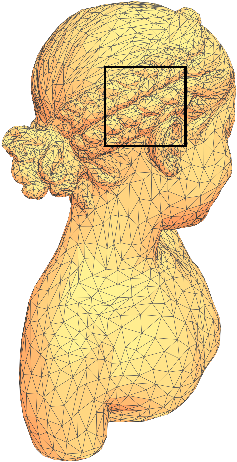
\includegraphics[width=0.8\textwidth]{figs/svg/bimba_wireframe_half_line_width_rect.png}
\end{minipage}%
\begin{minipage}[t]{0.7\textwidth}
\centering
   {   \setlength{\fboxsep}{0pt} \setlength{\fboxrule}{1pt} \fbox{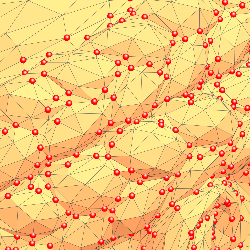
\includegraphics[width=0.35\textwidth]{figs/svg/bimba_saddle_closeup3.png}}}
    {   \setlength{\fboxsep}{0pt} \setlength{\fboxrule}{1pt} \fbox{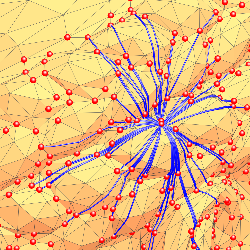
\includegraphics[width=0.35\textwidth]{figs/svg/bimba_SS_edges_closeup3.png}}}\\
    \makebox[0.35\textwidth]{saddle vertices}   \makebox[0.35\textwidth]{S-S edges} \\
   {   \setlength{\fboxsep}{0pt} \setlength{\fboxrule}{1pt} \fbox{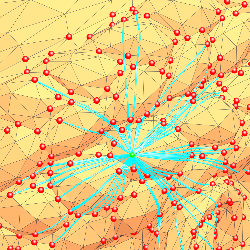
\includegraphics[width=0.35\textwidth]{figs/svg/bimba_NS_edges_3_closeup.png}}}
   {   \setlength{\fboxsep}{0pt} \setlength{\fboxrule}{1pt} \fbox{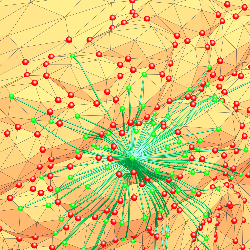
\includegraphics[width=0.35\textwidth]{figs/svg/bimba_NN_edges_closeup3.png}}}\\
    \makebox[0.35\textwidth]{N-S edges}  \makebox[0.35\textwidth]{N-N edges}
\end{minipage}
\vspace{-0.1in} \caption{The SVG on the $9$K-face Bimba. The saddle
vertices are drawn in red. For illustration purpose, we show only
the S-S, N-S and N-N edges incident to a vertex. } \label{fig:svg}
\end{figure}

Throughout this paper, we use $\{p,q\}$ to denote the undirected SVG
edge between $p$ and $q$, and $\|\{p,q\}\|$ to denote its length,
i.e., the geodesic distance $d(p,q)$, and $\|pq\|$ to denote the
Euclidean distance between $p$ and $q$.

\noindent\textbf{Remark.} If the mesh is viewed as a planet, the
vertices are the cities, and the geodesic path between two vertices
is a flight route. So the SVG is indeed a flight route map, which
covers every city on the planet. The saddle vertices are the hub
cities and the non-saddle vertices are the small cities. The S-S
edges are the major flight routes connecting the hubs. Each N-S edge
is a regional flight route connecting a small city to the nearest
hub. Each N-N edge is a local flight route between two nearby small
cities. Travelers moving between cities not served by direct flights
change planes en route to their destinations.


\subsection{Data Structure}
\label{subsec:datastructure}

We use the conventional incidence list to store the SVG. Each vertex
stores its incident edges (i.e., the direct geodesic paths) and each
edge stores one incident vertex and its length (i.e., the geodesic
distance).

\begin{small}
\begin{verbatim}
struct SVGVertex {
    int id;
    bool is_saddle;
    vector<SVGEdge> edges_incident_to_nonsaddle_vertices;
    vector<SVGEdge> edges_incident_to_saddle_vertices;
};
struct SVGEdge {
    int v2;
    double length, theta;
};
\end{verbatim}
\end{small}

%\vspace{-0.1in}
\pichskip{5pt}% Horizontal gap between picture and text
\parpic[r][t]{%
  \begin{minipage}{2.6in}
    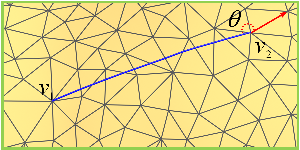
\includegraphics[width=2.5in]{figs/svg/path2_labels.png}
   \end{minipage}
}  In order to find the geodesic path, we also associate each SVG
edge with an angle $\theta$, which measures the direction of the
geodesic path with respect to its endpoint $v_2$. The reference
direction (the red edge in the figure on the right) is defined by
using $v_2$'s local information, such as its first incident mesh
edge. To obtain the geodesic path $\gamma(v_1,v_2)$, we back-trace
the curve from the endpoint $v_2$: with the reference direction and
the angle $\theta$, we can obtain the first segment of $\gamma$,
which is a straight line in triangle $T$, where $T$ is one of
$v_2$'s incident triangles. We then unfold $T$'s adjacent triangle -
say, $T'$ - into a common plane to extend the line to $T'$. We
repeat this unfolding until the geodesic path reaches $v_1$. As the
direct geodesic path does not pass through the saddle vertex, this
unfolding leads to a unique face/edge sequence and thus produces a
unique geodesic path. The procedure Backtrace$(e)$ is defined to
compute the direct geodesic path for an SVG edge $e$. The pseuocode
of the procedure Backtrace is shown in the Supplementary Material.

\subsection{Complexity Analysis}
\label{subsec:complexity}

The complexity of SVG obviously depends on the number of saddle
vertices and their distribution. Consider an extreme case in which
every vertex is either spherical or Euclidean (such as a convex
polyhedron or a developable surface), $V_S=\emptyset$ and
$|E_{NN}|={n\choose 2}$, since any geodesic path between two
vertices is direct. In this case, $S_3$ is dense and the whole SVG
is also dense.

\begin{figure}[htbp]
\centering
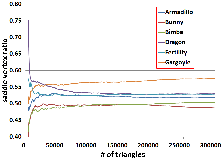
\includegraphics[width=0.8\textwidth]{figs/svg/saddle_ratio.png}
\vspace{-0.1in}
\caption{The saddle vertex ratio
$r=\frac{|V_S|}{|V|}$ is fairly stable with respect to the mesh
resolution and tessellation.}\label{fig:saddleratio}
\end{figure}
Fortunately, such extreme cases are rare in real-world applications
(see Section~\ref{sec:results} for the handling of such cases). We
tested the saddle vertex ratio $r=\frac{|V_S|}{|V|}$ on common
models of various resolutions. For each model, we generate triangle
meshes ranging from 1K triangles to 300K triangles. We have observed
that the value of $r$ may vary at low resolution, but it becomes
fairly stable when the mesh resolution is high. The typical value of
$r$ for real-world models ranges from $40\%$-$60\%$. See
Figure~\ref{fig:saddleratio}. Thanks to such a large proportion of
saddle vertices, most of the geodesic paths are indirect and the SVG
is a sparse graph. See Table~\ref{tab:SVGcomplexity}.

Through extensive experiments on a wide range of real-world models,
we have observed that the SVG exhibits a strong local structure. The
more details and complicated geometry the model has, the stronger
the local structure. To quantitatively measure the local structure
of the SVG, we consider the length of the SVG edges. We have
observed that the length of the direct geodesic path is inversely
proportional to the local vertex density (the number of vertices in
a region divided by the region's area), the higher the density, the
shorter the length, and vice versa. This is because the length of
the direct geodesic path depends on the number and distribution of
saddle vertices, which in turns depends on the mesh resolution. The
lower the resolution, the lower the density, the smoother the
surface, the less number of saddle vertices, and the longer the
direct geodesic paths. On the other hand, the higher the resolution,
the higher the vertex density, the more bumpy the surface, the
greater the number of saddle points, and the shorter the direct
geodesic paths. To obtain a resolution-independent measure, we
define the \textit{relative} SVG edge length $\widetilde{L}$, as the
ratio of the average length of the direct geodesic path and the
average mesh edge length. We also define the average SVG degrees for
the sub-graphs $S_1$, $S_2$ and $S_3$ to measure the SVG complexity:
\begin{displaymath}
D_{SS}=\frac{2|E_{SS}|}{|V_S|}, D_{NS}=\frac{|E_{NS}|}{|V_N|},
~\mathrm{and}~ D_{NN}=\frac{2|E_{NN}|}{|V_N|}.
\end{displaymath}
The coefficient $2$ in $D_{SS}$ and $D_{NN}$ is due to the double
counting of the $E_{SS}$ and $E_{NN}$ edges.


\pichskip{1pt}% Horizontal gap between picture and text
\parpic[r][t]{%
  \begin{minipage}{2.6in}
  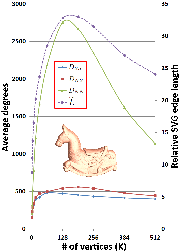
\includegraphics[width=2.5in]{figs/svg/horse_curve2.png}
   \end{minipage}
   }
   By investigating how the mesh complexity affects the SVG's local
structure and its complexity, we have observed that all the tested
real-world models exhibit an inverted U-shaped curve. The figure on
the right shows the curves for the Isidore Horse model. The
horizonal axis is the mesh complexity in terms of the number of
vertices, while the left and right vertical axes are the average SVG
degrees and the relative SVG edge length $\widetilde{L}$. When the
resolution is low, the model has almost no details and its body is
relatively smooth. Therefore, the degrees increase when the mesh
size is increased. When the resolution is sufficiently high, the
surface becomes bumpy due to the addition of details and has many
saddle vertices. Consequently, the S-S and N-S edges become shorter.
Furthermore, as each non-saddle vertex is surrounded by more saddle
vertices, and the direct geodesic path that originates from the
non-saddle vertices cannot reach too far away, the N-N edges are
also shorter. Therefore, the average degrees and the relative SVG
edge length $\widetilde{L}$ all tend to decrease at the high
resolution, which confirms that the SVG has strong local structure
when the mesh is of high resolution and has details. We also test
the SVG complexity and its local structure on the sphere model.
Because all vertices of the sphere are non-saddle, we add
geometrical noise to perturb the vertex position. We have found that
the SVG of the bumpy sphere exhibits the same characteristics as the
real-world models. See Figure~\ref{fig:sphere}.

Let $D=\max\{D_{SS},D_{NS},D_{NN}\}$ denote the maximal degree,
which is significantly less than the mesh size $D\ll n$ for
real-world models. Therefore, the SVG
is in general a sparse graph and the space complexity is $O(Dn)$.


\begin{figure}[htbp]\center
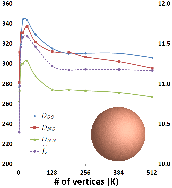
\includegraphics[height=3in]{figs/svg/sphere_01_without_vertical_labels.png}\hspace{0.05in}
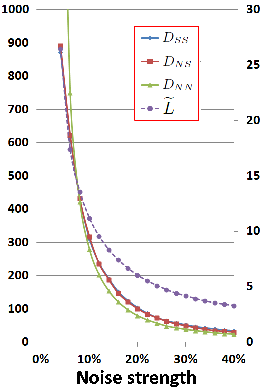
\includegraphics[height=3in]{figs/svg/sphere_noise_strength_scaled.png}\\
\makebox[2in]{(a)} \makebox[2in]{(b)} \vspace{-0.1in} \caption{(a)
Adding geometrical noise to the sphere, which moves each vertex in a
random direction by a uniform random distance $0$ to $10\%$ of
average edge length. (b) Increasing the noise strength makes the
sphere bumpier. As a result, both the average degrees and the
relative SVG edge length drop. The left and right vertical axes show
the average degrees and the relative SVG edge length
$\widetilde{L}$, respectively.} \label{fig:sphere}
\end{figure}

\section{SVG Construction}
\label{sec:exact}

The exact SVG contains \textit{all} direct geodesic paths, by which
we can compute the exact polyhedral distance between any two
vertices. In practice, we have found that an approximate\footnote{By
\textit{approximate}, we mean that the SVG's edge set is a subset of
the exact SVG's edge set. Each SVG edge $(p,q)$ in the approximate
SVG is still an exact direct geodesic path, which measures the
accurate geodesic distance between $p$ and $q$.} SVG with only a
subset of the direct geodesic paths can still lead to highly
accurate geodesic distance, but requires much less memory and is
more efficient to construct than the exact SVG.

\subsection{Parameter}

Our goal is to find a model and resolution insensitive parameter
that can intuitively and effectively control the SVG complexity.
Therefore, the maximal SVG edge length is not suitable, since it is
resolution-dependent. The relative SVG edge length cannot be used
either, since it is model dependent and may not be effective for
anisotropic meshes.

In our paper, we use the maximal number of mesh vertices covered by
a geodesic disk, denoted by $K$, as the parameter for controlling
the SVG complexity. Given a vertex $v\in V$, we consider a geodesic
disk $\odot(v,R)$ centered at $v$ with a radius $R$ that contains no
more than $K$ mesh vertices. Then the direct geodesic paths within
$\odot(v,R)$ are taken as the SVG edges.

There are a few advantages of using $K$ as the parameter. First, it
is a good measure of the computational cost. Computing the geodesic
disk $\odot(v,R)$ with the ICH/MMP algorithm takes the worst-case
$O(K^2 \log K)$ time and empirical $O(K^{1.5}\log K)$ time. Second,
the parameter $K$ \textit{directly} controls the number of direct
geodesic paths in the disk $\odot(v,R)$, which is insensitive to the
mesh resolution and tessellation. Let us examine the geodesic disks
$\odot(v,R)$ on a model $M$ in low resolution and high resolution,
denoted by $M_l$ and $M_h$, respectively. Fixing the value of $K$ of
course leads to geodesic disks of different radii on $M_l$ and
$M_h$. The radius $R_h$ is small, so the vertex density is high and
the direct geodesic paths are short. On the other hand, the radius
$R_l$ is big, so the vertex density is low and the direct geodesic
paths are long. Regardless of the size, the large and small disks
roughly contain the same number of direct geodesic paths originated
from $v$, since each geodesic path uniquely corresponds to a tangent
direction at $v$ and these tangent directions are intrinsic and
insensitive to the mesh resolution and tessellation. Therefore, the
parameter $K$ is model independent and can be used to control the
SVG complexity and analyze the time complexity of SVG construction.
\begin{table}[htbp]
\centering
\setlength\tabcolsep{2pt}
%\begin{small}
\begin{tabular}{|c||c|c|c|c|c|c|c|}
  \hline Model & $|V|$ & $r$ & $D_{SS}$ & $D_{NS}$ & $D_{NN}$ & $\widetilde{L}$ & ind.\% \\
  \hline Bimba & 74,764 & 51.6\% & 1279.1 & 1179.3 & 1168.6 & 30.4 & 96.9\%\\
  \hline Buddha & 488,217 & 56.1\% & 861.7 & 862.3 & 715.3 & 28.2 & 99.6\%\\
  \hline Bunny &  72,020  & 54.3\%  & 1029.8 & 998.2 & 1295.9 & 22.5 & 97.4\%\\
  \hline Dragon & 422,558 &  54.2\% & 1044.2 &  1043.6 &  924.1 & 29.8 & 99.5\%\\
  \hline Fertility & 29,994 &  52.3\% &  1483.4 & 1225.4 &  1172.1 & 26.4 & 91.6\%\\
  \hline Golfball & 122,882 & 31.0\% &  693.3  & 694.9 &  1586.4 & 20.9 & 98.2\%\\
  \hline Gargoyle & 349,998 & 58.0\% &  711.2  & 699.9 &  501.2 & 18.6 & 99.6\%\\
  \hline Kitten & 137,098 &  50.9\% &   991.3  & 914.6 &  981.8 & 20.2 & 98.6\%\\
  \hline Lucy  &  262,909 & 54.1\% & 390.5  & 325.6 &  1003.1 & 22.9 & 99.5\% \\
  \hline Ramses & 826,266 & 60.4\% &  365.8  & 322.8 & 204.6 & 12.5 & 99.9\%\\
  \hline
\end{tabular}
%\end{small}
\caption{Statistics of the SVG complexity on common models. The last column shows
the percentage of the indirect geodesic paths.}
\label{tab:SVGcomplexity}
\end{table}



\subsection{Computing Direct Geodesic Paths}
\pichskip{5pt}% Horizontal gap between picture and text
\parpic[r][t]{%
  \begin{minipage}{2.6in}
  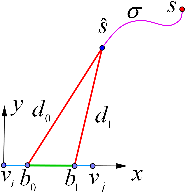
\includegraphics[width=2.575in]{figs/svg/window_tuple.png}
   \end{minipage}
}
To construct the SVG, we must compute the direct
geodesic paths. We adopt the half-edge data structure to store the
triangle mesh $M$. Each mesh edge is decomposed into two half-edges,
with opposite directions. A window $w$ associated to a half-edge
$e=(v_i,v_j)$ is a $5$-tuple $(b_0,b_1,d_0,d_1,\sigma)$, where
$b_0$, $b_1$ define the endpoints of $w$ ($b_0$ is closer to the
vertex $v_i$ where the half-edge is originated), $d_0$, $d_1$ are
the corresponding distances to the pseudosource, and $\sigma$ is the
geodesic distance from the source $s$ to the pseudo source
$\hat{s}$. We define the direct window as follows:

\noindent\textbf{Definition 6.} A window
$w=(b_0,b_1,d_0,d_1,\sigma)$ is said \textit{direct} if $\sigma=0$.

Intuitively, a direct window is an interval on a half-edge for which
there is a direct geodesic path from the source to any point in the
interval. To obtain the direct geodesic paths, we run the single
source geodesic algorithm (like the ICH or MMP algorithm) for each
vertex. The local structure of the SVG means that it is not
necessary for the geodesic algorithm to run for the entire mesh,
which would be very time-consuming. When a window $w$ propagates,
the value $\sigma$ of $w$'s child windows cannot decrease.
Therefore, the geodesic algorithm can simply stop when all direct
windows have been processed.

\subsection{Algorithm}

Our SVG construction algorithm is shown in Algorithm 1. For each
vertex $v_i\in V$, we run the procedure ComputeDirectGeodesicPaths
(see the Supplementary Material for the pseudocode), which takes
$v_i$ as the source and computes a geodesic disk $\odot(v_i,R)$ that
contains no more than $K$ vertices. Then all the directed geodesic
paths in $\odot(v_i,R)$ are taken to form the SVG edges.

Computing the direct geodesic paths is the bottleneck of the entire
SVG construction algorithm. In our implementation, we choose the ICH
algorithm to compute the direct geodesic paths due to its better
performance and less memory requirement than the MMP algorithm.
Moreover, the geodesic disks can be computed in parallel on the GPU:
the mesh data structure is accessible to all threads in the
read-only manner, and each thread of ComputeDirectGeodesicPaths
maintains its own data (for example, the windows and the priority
queues). To avoid the written conflicts, the thread for vertex $v_i$
produces \textit{directed} SVG edges originated from $v_i$. These
directed edges are then converted into undirected edges by checking
whether the opposite edges are available. See lines 5-9. Let $N$ be
the number of threads. The worst-case time complexity for computing
the direct geodesic paths is $O(nK^2\log K/N)$ and the empirical
time complexity is $O(nK^{1.5}\log K/N)$.

\begin{algorithm} [htbp]
\label{alg:construction} \caption{Constructing the SVG}
\begin{algorithmic}[1]
\Require A triangle mesh $M=(V,E,F)$ and the maximal number of
vertices $K$ in each geodesic disk;

\Ensure The saddle vertex graph $S$;

\If {each $v_i\in V$}

\State \textcolor{red}{\textbf{parallel}} $S_i \gets $
ComputeDirectGeodesicPaths($M$, $v_i$, $K$);

\EndIf

\State $S \gets \bigcup_{i=1}^{|V|} S_i$; \For {each edge $(s,t) \in
S$}
    \If{edge $(t,s) \notin S$ }
        \State add $(t,s)$ into $t$'s incident edges;
    \EndIf
\EndFor

\end{algorithmic}
\end{algorithm}

\begin{algorithm}[htbp]
\caption{Computing the SSSD Geodesic Distance}
\begin{algorithmic}[1]

\Require A triangle mesh $M=(V,E,F)$, the associated saddle vertex
graph $S=S_1\bigcup S_2\bigcup S_3$ and two vertices $p_1, p_2\in
V$.

\Ensure The geodesic distance $d(p_1,p_2)$.

\If{$p_1, p_2$ are direct neighbor} \State return $\|\{p_1,p_2\}\|$;
\EndIf \State $U \gets$ BidirectionalDijkstra$(\{V,E\}, p_1, p_2)$;
\If {$S$ is exact} \State $S_1'\gets S_1$; \For {i=1,2} \If
{$p_i\notin V_S$} \State $S_1' \gets S_1' \bigcup$\{$p_i$ and its
N-S edges\}; \EndIf \EndFor \State A$*$Dijkstra$(S_1',p_1,p_2,U)$;
\Else \State A$*$Dijkstra$(S_1\bigcup S_2\bigcup S_3,p_1,p_2,U)$;
\EndIf \State return $d_{p_1}(p_2)$;
\end{algorithmic}
\end{algorithm}


\section{Computing Discrete Geodesics Using SVG} \label{sec:geodesic}

\subsection{Dijkstra's Algorithm}
\label{subsec:dijkstra}

If the SVG is exact, according to Proposition 2, computing a
geodesic path on the mesh is equivalent to find a shortest path on
the SVG. On the other hand, the shortest path on an approximate SVG
provides an approximated geodesic path. On each occasion, we adopt
the Dijkstra algorithm~\cite{dijkstra1959note} to compute the shortest path
on the SVG.

Consider an undirected graph $G=(V,E)$ and a set of source points
$\mathfrak{S}\subset V$. The procedure Dijkstra$(G,\mathfrak{S})$ assigns each
vertex $v\in V$ a value $d(v)$, which is the shortest
distance from $v$ to the \textit{closest} source $s\in\mathfrak{S}$.

The Dijkstra's algorithm can be implemented with various data structures, such as queue, priority queue, binary heap, Fibonacci heap, etc.
We adopt the priority queue based Dijkstra's algorithm due to its simplicity and good performance.


We also adopt two variants of the Dijkstra search.
The procedure BidirectionalDijkstra$(G,p,q)$ runs two simultaneous Dijkstra searches on the graph $G$: one forward from $p$ and one backward from $q$, stopping when the two meet in the middle. The procedure returns the shortest distance between $p$ and $q$. The procedure A$*$Dijkstra$(G,p,q,U_{pq})$ is the A$*$ search~\cite{astar}~\cite{Goldberg:2005:CSP:1070432.1070455} on the graph $G$, where $U_{pq}$ is the heuristic estimate of the upper bound of the shortest distance between $p$ and $q$. The A$*$ search is guided by an estimate of the remaining distance to the destination.

\subsection{Single-source Single-destination (SSSD)}
\label{subsec:sssd}

 To compute the single-source single destination geodesic distance
$d(s,t)$, we adopt the widely used A$*$
search~\cite{astar}~\cite{Surazhsky_Etc:2005}, which searches only a
thin region surrounding the geodesic path $\gamma(s,t)$. Our SSSD
algorithm contains two steps: first, we use BidirectionalDijkstra on
the mesh edges to get the shortest distance $U_{st}$, which is the
\textit{upper} bound of the geodesic distance $d(s,t)$. Second, we
use the A$*$ search on the SVG guided by the upper bound $U_{st}$.
If the SVG is exact, the A$*$ search applies to the tier 1 graph
$S_1$, otherwise, the search applies to the entire saddle vertex
graph $S_1\bigcup S_2 \bigcup S_3$. During the bidirectional A$*$
search, we prune the search by allowing only the point $p$
satisfying the inequality $d_s(p)+\|pt\|\leq U_{st}$, where $d_s(p)$
is the shortest distance from the point $s$ to $p$ and $\|pt\|$ is
the Euclidean distance from $p$ to $t$. The figure on the right
shows an example of computing the single-source single-destination
geodesic distance on the $263$K-vertex Lucy model. The exact
polyhedral distance is $0.8188$. Given an approximate SVG with
$K=100$, the upper bound $U$ obtained by bidirectional Dijkstra
search is $0.8410$ and our computed geodesic distance is $0.8191$.
The bidirectional Dijkstra search region, colored in blue, contains
$89.5$K vertices, and the A$*$ search region, colored in red,
contains only $17.3$K vertices. Simply running the bidirectional
Dijkstra search on the SVG takes $0.078$s. However, running the
BidirectionalDijkstra on the mesh and the A$*$ search on the SVG
take only $0.028$s and $0.021$s, respectively. Therefore, the $A*$
search can improve the performance for the SSSD problem, especially
when $p$ and $q$ are far away.

The geodesic path $\gamma(p,q)$ can also be obtained easily. Let
$\{e_1,e_2,\cdots,e_k\}$ be the shortest path from $p$ to $q$ on the
SVG. Then the geodesic path $\gamma(p,q)=\bigcup_i$Backtrace$(e_i)$.
The time complexity to obtain $\gamma(p,q)$ is $O(k)$, where $k$ is
the number of triangles crossed by the path $\gamma(p,q)$.


\begin{figure*}[htbp] \centering
\makebox[\textwidth][c]{
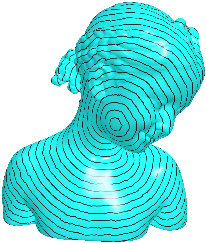
\includegraphics[height=1in]{figs/svg/bimba/bimba_FMM}
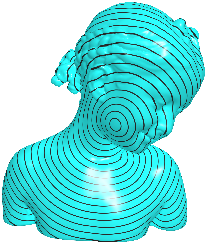
\includegraphics[height=1in]{figs/svg/bimba/bimba_heat}
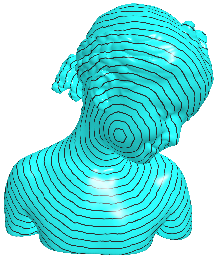
\includegraphics[height=1in]{figs/svg/bimba/bimba_K_6.png}
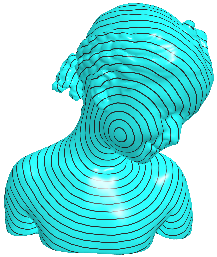
\includegraphics[height=1in]{figs/svg/bimba/bimba_K_16.png}
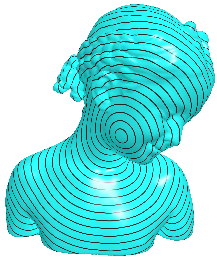
\includegraphics[height=1in]{figs/svg/bimba/bimba_K_30.png}
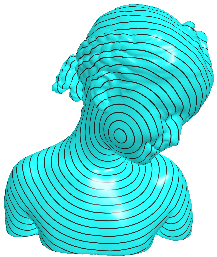
\includegraphics[height=1in]{figs/svg/bimba/bimba_K_50.png}
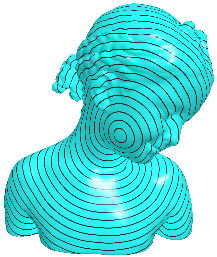
\includegraphics[height=1in]{figs/svg/bimba/bimba_K_100.png}
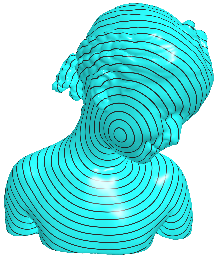
\includegraphics[height=1in]{figs/svg/bimba/bimba_exact.png}}\\
\makebox[\textwidth][c]{
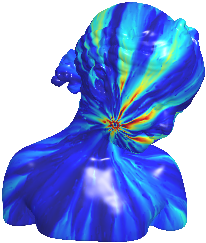
\includegraphics[height=1in]{figs/svg/bimba/bimba_FMM_error.png}
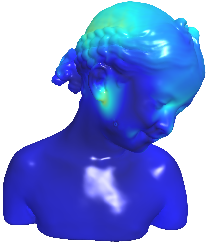
\includegraphics[height=1in]{figs/svg/bimba/bimba_heat_error_new.png}
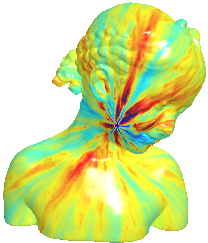
\includegraphics[height=1in]{figs/svg/bimba/bimba_K_8_error.png}
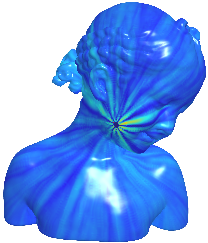
\includegraphics[height=1in]{figs/svg/bimba/bimba_K_16_error.png}
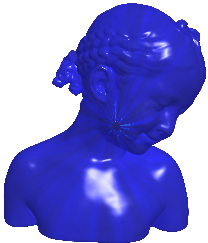
\includegraphics[height=1in]{figs/svg/bimba/bimba_K_30_error.png}
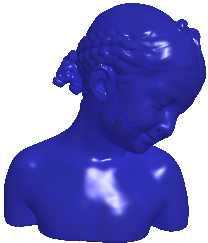
\includegraphics[height=1in]{figs/svg/bimba/bimba_K_50_error.png}
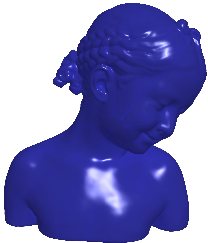
\includegraphics[height=1in]{figs/svg/bimba/bimba_K_100_error.png}
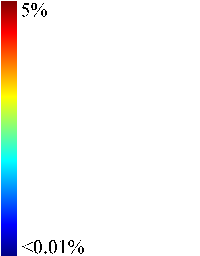
\includegraphics[height=1in]{figs/svg/bimba/colorbar.png}}\\

\begin{small}
\makebox[\textwidth][c]{
\makebox[1.2in]{FMM $\epsilon=0.78\%$} \makebox[0.8in]{Heat
$\epsilon=0.72\%$} \makebox[0.8in]{$(8, 1.96\%)$}
\makebox[0.8in]{$(16, 0.61\%$)} \makebox[0.8in]{$(30, 0.13\%)$}
\makebox[0.8in]{$(50,0.08\%$)} \makebox[0.8in]{$(100,0.035\%$)}
\makebox[0.8in]{exact}
}
\end{small}
\vspace{-0.01in} \caption{Visual comparison of the accuracy. The
2-tuple under the SVG result is $(K,\epsilon)$, where $\epsilon$ is
the mean relative error. $K=50$ leads to high quality result, where
the difference to the exact result is hardly visible.}
\label{fig:bimba}\end{figure*}

\subsection{Multiple-sources All-destinations (MSAD)}
\label{subsec:ssad}

The single-source and multiple-sources geodesic algorithms have the
same computational framework. If the SVG is exact, we first run the
Dijkstra search to the tier 1 graph $S_1$ and then update the
geodesic distance for each non-saddle vertex $q$ by using the
shortest distance from $q$'s saddle neighbors. Since it takes
$O(|E_{NS}|)$ time to update the geodesic distance for the
non-saddle vertices, the time complexity is
$O(|E_{SS}|\log|V_S|+|E_{NS}|)=O(Drn\log(rn)+D(1-r)n)$. If the SVG
is approximate, we run the Dijkstra search to the entire graph
$S_1\bigcup S_2\bigcup S_3$, which can reach all mesh vertices. The
time complexity is then $O((|E_{SS}|+|E_{NS}|+|E_{NN}|)\log |V|) =
O(Dn\log n)$.

\begin{algorithm}[htbp]
\caption{Computing the MSAD Geodesic Distance}
\begin{algorithmic}[1]

\Require A triangle mesh $M=(V,E,F)$, its saddle vertex graph
$S=S_1\bigcup S_2\bigcup S_3$ and the set of sources
$\mathfrak{S}=\{s_i\}_{i=1}^m$.

\Ensure $\forall t\in V$, $d(t)$ is the geodesic distance from $t$
to its closest source $s_i\in V$.

\If {$S$ is exact} \State $S_1'\gets S_1$; \For {each $s_i\in
\mathfrak{S}$} \If {$s_i\notin V_S$} \State $S_1' \gets S_1'
\bigcup$\{$s_i$ and its N-S edges\}; \EndIf \EndFor

\State Dijkstra$(S_1', \mathfrak{S})$; \For {each $q\in V_N$}
    \State $d(q)=\min_{t\in \mathcal{S}(q)} \{d(t)+\|\{t,q\}\|\}$;
\EndFor \Else \State Dijkstra$(S_1\bigcup S_2\bigcup S_3,
\mathfrak{S})$; \EndIf
\end{algorithmic}
\end{algorithm}

\section{Experimental Results }
\label{sec:results}

\noindent\textbf{Performance.} Due to the computation of the exact
geodesic paths, the SVG construction is expensive. Fortunately, the
SVG can be constructed in a parallel manner. We implemented the SVG
construction algorithm on CUDA 5.0 and run it on an Nvidia Tesla K20
graphics card with 2496 CUDA cores and 5GB memory to produce all the
SVGs used in this paper. Take the $263$K-vertex Lucy for example. It
takes $3.68$s, $12.84$s, and $381.1$s to construct the SVG with
$K=30$, $100$, and $1000$, respectively. The computed SVGs are
stored in a binary file format, which will be used in the Dijkstra
search.

We implemented the priority queue based Dijkstra algorithm and its
two variants, bidirectional Dijkstra search and A$*$ search, and
tested our algorithms, SSSD, SSAD, MSAD on an Intel Xeon 2.66GHz CPU
machine. Only a single core was used to compute the various types of
geodesic distances. Table~\ref{tab:meshcomplexity} shows the mesh
complexity and performance of our method and other approximate
algorithms. Since all the other geodesic algorithms are CPU-based,
we also show the CPU pre-computation time of our method to make a
fair comparison. We have found that our CPU-based program is usually
$10$ to $40$ times slower than the parallel program on the Tesla K20
GPU.

Our method solves the SSAD and MSAD geodesic distances in a unified
framework. The MSAD algorithm allows us to compute the geodesic
Voronoi diagram and the geodesic distances to curve sources. See
Figure~\ref{fig:gvd}.

\begin{table*}[htbp]
%\renewcommand{\arraystretch}{1.2}% Wider
\caption{Statistics of speed and accuracy. $T_p^{c}$ (resp.
$T_p^{g}$): time for pre-computing on the CPU (resp. GPU); $T$: time
for solving the single-source geodesic distance; $\epsilon$: mean
relative error; $S$: memory required for storing SVG.} \centering
\setlength{\tabcolsep}{1.75pt}
\begin{tiny}
\begin{tabular}{|l||c||c|c|c|c|c|c|c|c|c|c|c|c|c|c|c|c|c|c|c|c|c|c|c|c|}
\hline
         Model ($|V|$) & ICH          & \multicolumn{2}{|c|}{FMM}
                       & \multicolumn{3}{|c|}{GTU ($m=3000$)} & \multicolumn{3}{|c|}{Heat Method ($t=h^2$)}
                       & \multicolumn{5}{|c|}{SVG ($K=100$)}
                       & \multicolumn{5}{|c|}{SVG ($K=1000$)}\\
                       \cline{2-2} \cline{3-4}
                       \cline{5-7} \cline{8-10}
                       \cline{11-15} \cline{16-20}

                       & $T$ (s) & $T$ (s) & $\epsilon$
                       & $T_p^c$ (s) & $T$ (s) & $\epsilon$ & $T_p^c$ (s) & $T$ (s) & $\epsilon$
                       & $S$ (Mb) & $T_p^c$ (s) & $T_p^g$ (s) & $T$ (s) & $\epsilon$
                       & $S$ (Mb) & $T_p^c$ (s) & $T_p^g$ (s) & $T$ (s) & $\epsilon$
                       \\
\hline Armadillo (173K) & 10.45 & 7.57 & 1.34\% &  3878 & 7.28 & 0.27\%& 2.28 & 0.26 & 0.92\% & 313.3 & 168.1 &8.82  & 0.29& 0.047\% & 1905 & 4895 & 247.1 & 0.72 & 0.0011\%\\
\hline Bunny (72K) & 6.33& 2.45 & 0.66\%&  2315 & 2.03 & 0.26\% & 1.09 & 0.10 &0.85\% & 124.4 & 68.0 &3.77 & 0.10& 0.041\% & 966.5 & 2041 & 105.5 & 0.22 & 0.0011\%\\
\hline Fertility (30K)& 1.90 & 0.47 &1.18\%  & 684 & 0.63 & 0.11\% & 0.45& 0.03 & 0.56\%& 54.4 & 29.1 &1.69 & 0.04& 0.041\% & 417.8 & 843.3 & 43.9 & 0.12 & 0.0012\%\\
\hline Gargoyle (350K) & 80.1 & 46.1&1.57\% &  28743 & 16.83 & 0.29\% & 12.03& 0.53 & 0.96\%& 633.2 & 340.1 &18.20 & 0.44& 0.048\% & 5282 & 9911 & 508.7 & 1.41 & 0.0009\%\\
\hline Lucy (263K)& 18.2& 15.8 & 1.78\% &  6872 & 11.69 & 0.23\% & 8.10& 0.37 &0.91\%  & 477.8 &259.4 &12.84  & 0.39& 0.056\% & 3957 & 7451 & 381.1 & 0.97 & 0.0016\%\\
\hline Dragon (3M) & 194.3 & 155.1 & 1.87\% &  65599 & 128.1 & 0.31\% & \multicolumn{3}{|c|}{Out of memory} & 5057 & 2894 & 151.2 & 4.11 & 0.048\% & \multicolumn{5}{|c|}{Out of memory}\\
\hline
\end{tabular}
\end{tiny}\label{tab:meshcomplexity}
\end{table*}

\noindent\textbf{Accuracy.} We compare our approximate geodesic
distance to the exact polyhedral
distance~\cite{Mitchell_Etc:1987}~\cite{Xin_Wang:2009} and measure
the relative difference $|d(x,y)-\widetilde{d}(x,y)|/d(x,y)$, where
$d(x,y)$ and $\widetilde{d}(x,y)$ are the exact and approximate
distances, respectively. We report the maximal, root-mean-square
error, and mean relative differences. As Figure~\ref{fig:K} shows,
increasing $K$ makes an approximate SVG approaching the exact SVG.
Figure~\ref{fig:K}(b) plots the mean relative error as function of
$K$. Figure~\ref{fig:K}(c) shows the error vs $K$ curves with
respect to the mesh resolution and tessellation. We down-sample the
144K-face Bunny to 6 isotropic and anisotropic meshes. All the error
vs $K$ curves exhibit the same pattern with slightly different
ranges. Figure~\ref{fig:buddha} shows the Happy Buddha model from a
low-resolution mesh with many obtuse triangles to a high-resolution
mesh with regular triangulation. The same parameter $K=30$ produces
consistently high quality results for all three meshes. This again
justifies that the parameter $K$ is resolution and triangulation
insensitive. Figure~\ref{fig:bimba} shows the geodesic distances on
the Bimba with various $K$. Figure~\ref{fig:results} shows the
results on the Bunny and the Armadillo. See more results in the
Supplementary Material.

Following~\cite{heat_tog}, we also examine the errors relative to
the mean edge length $h$ on the unit sphere, where the analytic
geodesic distance is available. We observe that the heat method
provides a linear convergence and the exact polyhedral distance
converges quadratically. As shown in Figure~\ref{fig:convergence},
our method with $K=500$ has the same quadratic convergence rate as
the exact polyhedral distance for large mean edge length $h$, while
the convergence speed becomes slower when $h$ is small. This result
is not a surprise. Our SVG with a large $K$ does compute the
\textit{exact} polyhedral distance when the mesh resolution is low,
since the SVG is exact and contains all direct geodesic paths. On
the other hand, when the mesh resolution is high and the parameter
$K$ is relative small, the corresponding SVG becomes approximate
since it contains only a subset of the direct geodesic paths and the
resulting geodesic distance is approximate. An interesting
observation shows that the approximate SVG converges slightly faster
than the exact polyhedral distance when the mean edge length
$h\in[0.03,0.15]$. This is due to the fact that the approximate SVG
always produces a \textit{longer} distance than the exact polyhedral
distance on arbitrary meshes. On the mesh representing the sphere,
the exact polyhedral distance is always less than the analytic
geodesic distance. Therefore, when the mesh resolution is in the
aforementioned range, the distance produced by the SVG tends to be
more accurate than the exact polyhedral distance.


The existing approximation algorithms usually work well for smooth
surfaces. However, their accuracy could be very low if the models
have rich features. In sharp contrast, our method works remarkably
well for real-world models with geometric features, since our method
does take advantage of these details: the richer the geometric
features, the stronger the local characteristic of the discrete
geodesic is, the more accurate SVG we can construct (with a fixed
$K$), and the \textit{more} accurate geodesic we obtain. Our result
on the 1.5M-face Dragon has mean relative error less than $0.04\%$.
Comparing to the result of the exact algorithm, such a small error
is not visually noticeable. See Figure 1.

\noindent\textbf{Metric.} It is well known that given an undirected
connected graph $G$, the set $V$ of vertices of $G$ forms a metric
space by defining $d(x,y)$ to be the length of the shortest path
connecting the vertices $x$ and $y$. Since we compute the geodesic
distance by using the shortest path distance on the SVG, the
resulting distance is guaranteed to be a metric, i.e., satisfying
the symmetry condition and triangle inequality. All the other
approximate algorithms, such as the FMM, the AMMP algorithm, the
heat method and the GTU method, exhibit violations of metric
properties.

\begin{figure*}[htbp]
\centering
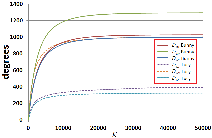
\includegraphics[height=1.3in]{figs/svg/bunny_lucy_k_curve.png}
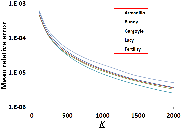
\includegraphics[height=1.3in]{figs/svg/error_all_models.png}
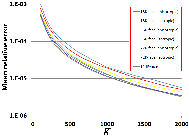
\includegraphics[height=1.3in]{figs/svg/bunny_error.png}\\
\makebox[2.2in]{(a) Degrees vs $K$}\makebox[2.2in]{(b) Mean relative
error vs $K$}\makebox[2.2in]{(c) Mean relative error vs
$K$}\vspace{-0.1in} \caption{The parameter $K$ effectively controls
the SVG complexity and the accuracy of the approximate geodesic
distance. (a) A sufficiently large $K$ produces the exact SVG. (b)
The mean relative error as a function of $K$ on various models. (c)
The mean relative error as a function of $K$ on Bunny of various
resolutions and tessellations. } \label{fig:K}
\end{figure*}

\noindent\textbf{Convex or developable surfaces.} Our method works
remarkably well for real-world models which contain large number of
saddle vertices. However, our method is not efficient for computing
geodesic distances on convex polyhedrons and developable surfaces,
which do not have saddle vertices at all. Therefore, every geodesic
path is direct and the associated corresponding SVG is a dense graph
with $|E_{NN}|={n\choose 2}$ and $D=n$. It is very expensive to
construct and store such a dense graph. Alternatively, one can seek
other efficient techniques for these special cases. Shreiber and
Sharir~\cite{Schreiber:2006} presented an optimal time $O(n\log
n)$ algorithm to compute the single source geodesic on convex
polyhedra. For the developable surfaces, one can adopt the FMM with
spherical wavefront propagation~\cite{sphericalwavefront}, which can
compute the exact polyhedral distance in $O(n\log n)$ time too.




\begin{figure}[htbp]
\centering
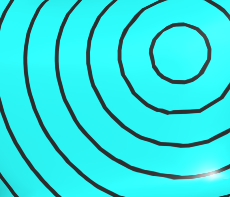
\includegraphics[width=0.3\textwidth]{figs/svg/path/exactfield3}
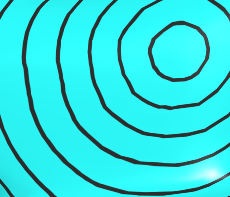
\includegraphics[width=0.3\textwidth]{figs/svg/path/heatfield3}
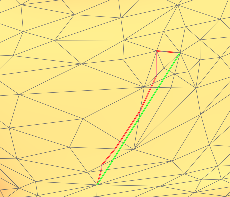
\includegraphics[width=0.3\textwidth]{figs/svg/path/pathtracing3}\\
\makebox[0.3\textwidth]{Our result} \makebox[0.3\textwidth]{Heat method} \makebox[0.3\textwidth]{Geodesic paths}\\
\vspace{-0.1in} \caption{The SVG method computes the geodesic path
by unfolding a sequence of triangles, which is stable and accurate.
The other approximate algorithms computes the geodesic path by
tracing the gradient of the distance, which is sensitive to the
triangulation. The geodesic paths obtained by our method and the
heat method are colored in green and red,
respectively.}\label{fig:path}
\end{figure}

\noindent\textbf{Geodesic path.} Like the other approximate
algorithms, the heat method computes the geodesic path by tracing
the gradient of the distance function. Note that the discrete
gradient operator computes the exact gradient only if the underlying
function is piecewise linear. However, the distance function is
non-linear. Therefore, the gradient tracing usually leads to
incorrect result when the triangulation is poor. Our method computes
the geodesic path by triangle unfolding. Let $\gamma(s,t) \in M$ be
the geodesic path on $M$ and $\{p_0,p_1\}, \{p_1,p_2\}, \cdots,
\{p_k,p_{k+1}\}$ be the corresponding shortest path on the SVG,
where $p_0=s$ and $p_{k+1}=t$. Then the procedure
$\bigcup_{i=0}^{k}$Backtrace$(\{p_i,p_{i+1}\})$ can recover the
geodesic path $\gamma(s,t)$ accurately. See Figure~\ref{fig:path}.

\noindent\textbf{Scalability.} It is worth noting that our method
has advantages in terms of the scalability. Fixing the parameter
$K$, both the time and space complexities of the pre-computing are
linear to the number of vertices $n$. The direct geodesic paths are
computed on the GPU, and the graph is formed on the CPU. Our
GPU-based program on Tesla K20 can process a mesh with up to fifty
(resp. twelve) million triangles when $K=30$ (resp. $100$). If the
entire pre-computation is done on the CPU, our program can process
even larger meshes, since the CPU RAM is usually much bigger than
the GPU RAM. Note that the heat method prefactors the Laplacian
matrix, which has non-linear time and space complexities. Given a PC
with 12GB CPU memory, the existing open-source Cholesky
factorization package
(e.g.,Cholmod~\cite{Davis:2009:DSS:1462173.1462176}) can process
meshes with up to five million triangles.

\noindent\textbf{Domain.} The heat method takes advantages of the
well-established discrete Laplacian, and can easily adapt to a
variety of geometric domains, including high-degree nonplanar
polygonal meshes, and point clouds. Our method is limited to the
triangle meshes.

\section{Summary}\label{sec:summary}

The proposed SVG method is highly efficient, accurate, numerically
stable and robust to the mesh resolution and tessellation. Unlike
the other approximate algorithms that usually produce less accurate
results for models with rich geometric features, our method works
remarkably well for such models. The user can intuitively control
the accuracy as well as the SVG complexity by the parameter $K$,
which specifies the maximal number of points in a geodesic disk. The
parameter $K$ is independent to the scale, model, mesh resolution
and tessellation. Moreover, our method guarantees the computed
distance is a metric. Experiments on a wide range of real-world
models demonstrate that our method significantly outperforms the
existing approximate algorithms in terms of accuracy and speed.

\begin{figure}[htbp]
\centering
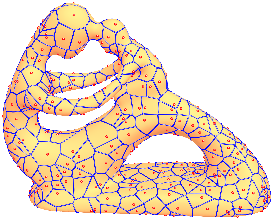
\includegraphics[height=2.6in]{figs/svg/GVD/fertility_nf60k_voronoi_500.png}
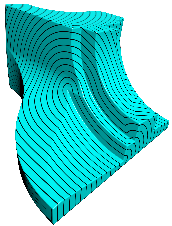
\includegraphics[height=2.6in]{figs/svg/offset/fandisk.png}\\
\makebox[0.45\textwidth]{(a) Geodesic Voronoi diagram} \makebox[0.45\textwidth]{(b)
Curve sources}
\caption{The MSAD algorithm allows us to compute the geodesic
Voronoi diagram and the geodesic distances to curve sources. (a) 500
random selected vertices are used as the seeds for the Voronoi
diagrams. (b) The vertices on the curves are used as the sources.}
\label{fig:gvd}
\end{figure}


\begin{figure}[htbp]
\centering
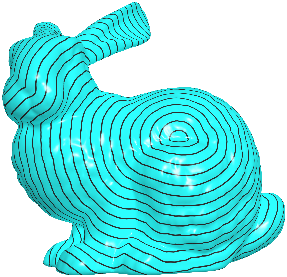
\includegraphics[width=0.25\textwidth]{figs/svg/bunny_SVG_small_front.png}
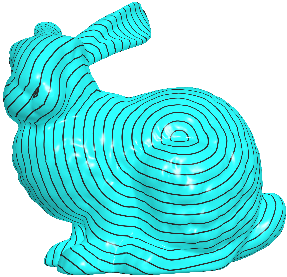
\includegraphics[width=0.25\textwidth]{figs/svg/bunny_GTU_1k_front.png}
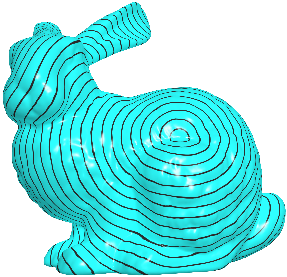
\includegraphics[width=0.25\textwidth]{figs/svg/bunny_heat_front.png}\\
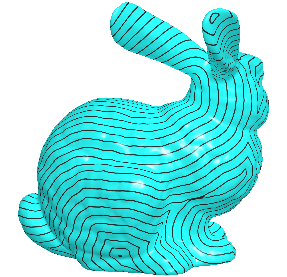
\includegraphics[width=0.25\textwidth]{figs/svg/bunny_SVG_small_back.png}
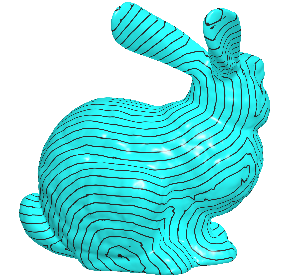
\includegraphics[width=0.25\textwidth]{figs/svg/bunny_GTU_1k_back.png}
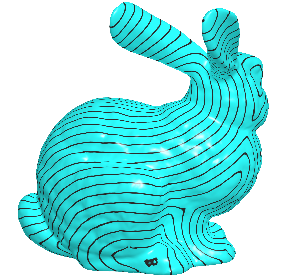
\includegraphics[width=0.25\textwidth]{figs/svg/bunny_heat_back.png}\\
\begin{small}
  \makebox[0.25\textwidth]{SVG $K=30$, $0.045$s}      \makebox[0.25\textwidth]{GTU $m=3000$, $2.03$s}    \makebox[0.25\textwidth]{Heat $t=h^2$, $0.10$s}\\
  \makebox[0.25\textwidth]{$(0.253\%, 0.17\%,0.12\%)$} \makebox[0.25\textwidth]{$(0.97\%,0.45\%,0.26\%)$} \makebox[0.25\textwidth]{$(1.84\%, 0.93\%,0.83\%)$}
\end{small}
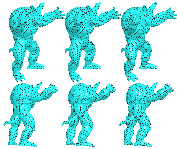
\includegraphics[width=0.9\textwidth]{figs/svg/armadillo_three.png}\\
\begin{small}
 \makebox[0.25\textwidth]{SVG $K=100$, $0.29$s}      \makebox[0.25\textwidth]{GTU $m=3000$, $7.28$s}                \makebox[0.25\textwidth]{Heat $t=h^2$, $0.26$s} \\
 \makebox[0.25\textwidth]{$(0.13\%,0.055\%,0.047\%)$}  \makebox[0.25\textwidth]{$(0.59\%, 0.44\%, 0.27\%)$} \makebox[0.25\textwidth]{$(1.96\%, 1.05\%, 0.92\%)$}\\
\end{small}\vspace{-0.1in}
\caption{Experimental results. The 3-tuple shows max relative error,
root-mean-square relative error and mean relative error. The exact
results are not shown here since our results are visually identical
to the exact results. } \label{fig:results}
\end{figure}

\begin{figure}[htbp]
\centering
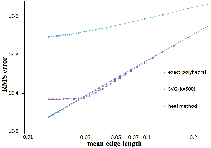
\includegraphics[width=0.995\linewidth]{figs/svg/convergence_rate2.png}
\caption{Convergence of distance functions on the unit sphere. The
vertical and horizontal axes show the logarithm of the
root-mean-square error and the mean edge length respectively. The
exact polyhedral distance converges quadratically while the heat
method converges linearly. Our method has the same convergence rate
as the exact algorithm when the mesh resolution is low and $K$ is
big. The convergence rate becomes linear when the mesh resolution is
sufficiently high.}
\label{fig:convergence}
\end{figure}

\begin{figure}[htbp]
\centering
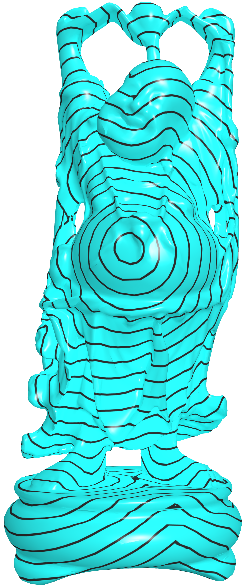
\includegraphics[width=0.3\textwidth]{figs/svg/buddha_nf40k_svg_RMS_0_16.png}
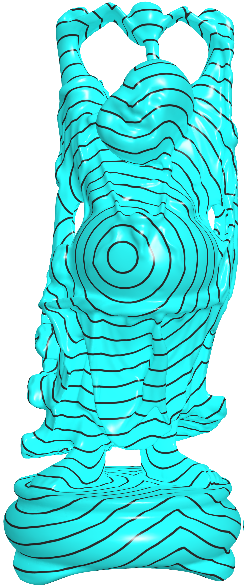
\includegraphics[width=0.3\textwidth]{figs/svg/buddha_nf300k_svg_RMS_0_11.png}
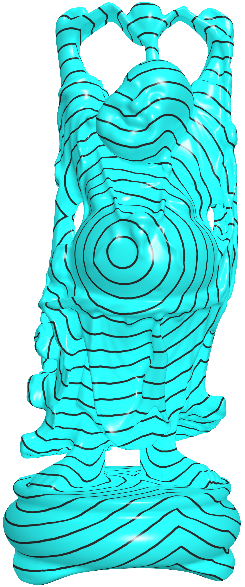
\includegraphics[width=0.3\textwidth]{figs/svg/buddha_nf600k_SVG_RMS_0_12.png}\\
 { \setlength{\fboxsep}{0pt} \setlength{\fboxrule}{1pt}\fbox{\includegraphics[width=0.3\textwidth]{figs/svg/buddha_nf40k_base_closeup.png}}}
 {   \setlength{\fboxsep}{0pt} \setlength{\fboxrule}{1pt}\fbox{\includegraphics[width=0.3\textwidth]{figs/svg/buddha_nf300k_base_closeup.png}}}
 {   \setlength{\fboxsep}{0pt}
 \setlength{\fboxrule}{1pt}\fbox{\includegraphics[width=0.3\textwidth]{figs/svg/buddha_nf600k_base_closeup.png}}}\\
\begin{scriptsize}
\makebox[0.3\textwidth]{$(0.37\%, 0.15\%, 0.11\%)$} \makebox[0.3\textwidth]{$(0.35\%,0.13\%,0.11\%)$} \makebox[0.3\textwidth]{$(0.29\%,0.13\%,0.11\%)$}\\
\end{scriptsize}
\vspace{-0.1in} \caption{The SVG method is numerically stable and
the approximated geodesic distances are insensitive to the mesh
tessellation and resolution. From left to right: 40K-face, 300K-face
and 600K-face. The same parameter $K=30$ applying to all three cases
produces consistently high quality results. } \label{fig:buddha}
\end{figure} 



\section{Introduction}
\label{sec:introduction}

Centroidal Voronoi tessellation (CVT) is a special type of Voronoi
diagram (VD) such that the generating point of each Voronoi cell is
also its center of mass~\cite{Du:1999:CVT:340312.340319}. The CVT
has broad applications in computer graphics, such as meshing,
stippling, sampling, etc. Although the CVT in Euclidean space has
been extensively studied, relatively little progress has been
reported towards computing the CVT on curved surfaces. A key step in
computing the CVT is to construct the Voronoi diagrams in each
iteration. It is fairly simple to construct the
 Voronoi diagrams in Euclidean space (e.g. $\mathbb{R}^2$ and
$\mathbb{R}^3$), since many efficient algorithms and software tools
are readily available. However, it is technically challenging to
compute VD on curved surfaces. Some researchers tackle this
challenge by computing the restricted Voronoi
diagrams~\cite{DBLP:journals/cgf/YanLLSW09}, which is the
intersection between the input mesh and the Voronoi diagram in
$\mathbb{R}^3$. These approaches are embedding space dependent and
may fail on models with complicated geometry and/or topology. Others
adopt the global parametrization to map the surface to the
parametric domain, such as Euclidean plane $\mathbb{E}^2$, the
sphere $\mathbb{S}^2$,  or hyperbolic disk $\mathbb{H}^{2}$, in
which the 2-dimensional CVT is
computed~\cite{DBLP:journals/cad/ShuaiGJ13}. It is known that
parameterizing models with complicated geometry and/or topology is
computationally expensive and often suffers serious numerical
issues. To our knowledge, there is no method for computing the CVT
on \textit{arbitrary} surfaces.

  \begin{figure}[htbp]
  \centering
  \includegraphics[width=2.550in]{figs/cvt/pegaso_nf667k_seed3000_small_whole_new.png}
  \caption{Our intrinsic method can compute a high-quality centroidal Voronoi tessellation on model with complicated geometry and topology. The CVT on the Pegaso model was created by 3000 sites. }
  \label{fig:teaser}
  \end{figure}

To tackle the above-mentioned challenge, this chapter presents two
\textit{intrinsic} algorithms for computing the centroidal Voronoi
tessellation on arbitrary triangle meshes. Our first algorithm
adopts the Lloyd framework, which iteratively moves the generator of
each geodesic Voronoi diagram to its mass center. Based on the
discrete exponential map, our method can efficiently compute the
Riemannian center and the center of mass for any geodesic VD. Our
second algorithm uses the L-BFGS method (limited-memory BFGS), which
uses the CVT energy function and its gradients to approximate the
Hessian matrix. The L-BFGS method has better performance due to its
super-linear convergence rate. Thanks to the intrinsic feature, our
methods are independent of the embedding space, and work well for
models with arbitrary topology and complicated geometry, where the
existing extrinsic approaches often fail. Figure~\ref{fig:teaser}
shows our result on the genus-5 Pegaso model. Moreover, our methods
are insensitive to the mesh resolution and tessellation, and can be
applied to surfaces embedded in arbitrary dimensional space. The
promising experimental results demonstrate the efficacy of our
methods.

The rest of the chapter is organized as follows.
Then Section~\ref{sec:lloyd} and section~\ref{sec:lbfgs} presents our intrinsic Lloyd and L-BFGS CVT algorithms in details. Section~\ref{sec:results} shows the experimental results, compares our method to the existing techniques and discusses its advantages and limitations. Finally, Section~\ref{sec:conclusion} concludes the chapter.


\section{The Lloyd Framework} \label{sec:lloyd}

\subsection{Overview} \label{subsec:overview}
Let $M=(V,E,F)$ be a triangle mesh representing a 2-manifold
surface, where $V$, $E$ and $F$ are the set of vertices, edges and
faces, respectively. Let $S=\{s_i|s_i\in M, i=1,\cdots, m\}$ denote
the set of sites on $M$.

Our algorithm adopts the Lloyd framework, which iteratively computes the geodesic CVT on meshes.
For each iteration, we first compute the multiple-source-all-destination geodesic distance with the sites $s_i$, $i=1,\cdots,m$, as the sources.
This geodesic distance field on $M$ induces a geodesic Voronoi diagram.
Then for each geodesic Voronoi cell, say $\Omega_j\in M$, we compute its Riemannian center $r_j$, which is defined as the average of its corners.
 Next, we compute the exponential map $\exp(r_j)$ at the Riemannian center $r_j$, and map the Voronoi cell $\Omega_j$ to the tangent plane $T_{r_j}$, on which we can compute the center of mass $c_j$. Finally, we map the mass center from the tangent plane to the mesh using the exponential map $\exp(r_j)$. We update each site $s_i$ to the new mass center and then repeat the above-mentioned procedure until the offsets of the sites are below the user-specified threshold.


\begin{algorithm} [t]
\label{alg:construction} \caption{Intrinsic computation of centroidal
Voronoi tessellation on meshes}
\begin{algorithmic}[1]
\Require A triangle mesh $M=(V,E,F)$, the set of sites
$S=\{s_i|s_i\in M, i=1,\cdots, m\}$ and the convergence threshold
$\epsilon$;

\Ensure The centroidal Voronoi tessellation on $M$;

\State \textbf{do}

\State ~~~~Compute geodesic distance field with $\{s_i\}_{i=1}^{m}$ as sources;

\State ~~~~Form the geodesic Voronoi diagram;

\State ~~~~\textbf{for} {$i=1$ to $m$} \textbf{do}

\State ~~~~~~~~Compute the Riemannian center $r_i$ for Voronoi cell $\Omega_i$;

\State ~~~~~~~~Compute the center of mass $c_i$ for $\Omega_i$;

\State ~~~~~~~~$d_i\gets d(s_i,c_i)$;

\State ~~~~~~~~$s_i\gets c_i$;

\State ~~~~\textbf{end for}

\State \textbf{while} $\frac{\sum_{i=1}^{m}d_i}{m}>\epsilon$

\end{algorithmic}
\end{algorithm}

\begin{figure}[htbp]
\centering
\makebox[\textwidth][c]{
\includegraphics[width=0.15\textwidth]{figs/cvt/eight_itr1.png}
\includegraphics[width=0.15\textwidth]{figs/cvt/eight_itr2.png}
\includegraphics[width=0.15\textwidth]{figs/cvt/eight_itr4.png}
\includegraphics[width=0.15\textwidth]{figs/cvt/eight_itr8.png}
\includegraphics[width=0.15\textwidth]{figs/cvt/eight_itr16.png}
\includegraphics[width=0.15\textwidth]{figs/cvt/eight_itr32.png}
\includegraphics[width=0.15\textwidth]{figs/cvt/eight_itr64.png}
\includegraphics[width=0.15\textwidth]{figs/cvt/eight_itr100.png}}\\
\makebox[\textwidth][c]{
\makebox[0.15\textwidth]{iteration \#1}
\makebox[0.15\textwidth]{\#2}
\makebox[0.15\textwidth]{\#4}
\makebox[0.15\textwidth]{\#8}
\makebox[0.15\textwidth]{\#16}
\makebox[0.15\textwidth]{\#32}
\makebox[0.15\textwidth]{\#64}
\makebox[0.15\textwidth]{\#100}}\\
\makebox[\textwidth][c]{
\makebox[0.15\textwidth]{$6.687\times 10^{-4}$}
\makebox[0.15\textwidth]{$4.425\times 10^{-4}$}
\makebox[0.15\textwidth]{$3.922\times 10^{-4}$}
\makebox[0.15\textwidth]{$3.536\times 10^{-4}$}
\makebox[0.15\textwidth]{$3.392\times 10^{-4}$}
\makebox[0.15\textwidth]{$3.319\times 10^{-4}$}
\makebox[0.15\textwidth]{$3.284\times 10^{-4}$}
\makebox[0.15\textwidth]{$3.271\times 10^{-4}$}}\\
\makebox[\textwidth][c]{
\includegraphics[width=0.15\textwidth]{figs/cvt/eight_lbfgs_itr1.png}
\includegraphics[width=0.15\textwidth]{figs/cvt/eight_lbfgs_itr2.png}
\includegraphics[width=0.15\textwidth]{figs/cvt/eight_lbfgs_itr4.png}
\includegraphics[width=0.15\textwidth]{figs/cvt/eight_lbfgs_itr8.png}
\includegraphics[width=0.15\textwidth]{figs/cvt/eight_lbfgs_itr16.png}
\includegraphics[width=0.15\textwidth]{figs/cvt/eight_lbfgs_itr32.png}
\includegraphics[width=0.15\textwidth]{figs/cvt/eight_lbfgs_itr64.png}
\includegraphics[width=0.15\textwidth]{figs/cvt/eight_lbfgs_itr100.png}}\\
\makebox[\textwidth][c]{
\makebox[0.15\textwidth]{iteration \#1}
\makebox[0.15\textwidth]{\#2}
\makebox[0.15\textwidth]{\#4}
\makebox[0.15\textwidth]{\#8}
\makebox[0.15\textwidth]{\#16}
\makebox[0.15\textwidth]{\#32}
\makebox[0.15\textwidth]{\#64}
\makebox[0.15\textwidth]{\#100}}\\
\makebox[\textwidth][c]{
\makebox[0.15\textwidth]{$6.687\times 10^{-4}$}
\makebox[0.15\textwidth]{$4.400\times 10^{-4}$}
\makebox[0.15\textwidth]{$3.736\times 10^{-4}$}
\makebox[0.15\textwidth]{$3.397\times 10^{-4}$}
\makebox[0.15\textwidth]{$3.287\times 10^{-4}$}
\makebox[0.15\textwidth]{$3.259\times 10^{-4}$}
\makebox[0.15\textwidth]{$3.249\times 10^{-4}$}
\makebox[0.15\textwidth]{$3.245\times 10^{-4}$}}
\caption{Iteratively computing geodesic CVT on meshes. Row
1: the Lloyd algorithm; Row 2: the L-BFGS algorithm.}
\label{fig:eight}
\end{figure}

\begin{figure}[htbp]
\centering
\includegraphics[width=0.23\textwidth]{figs/cvt/eight_GVD_seed100_distance_field.png}
\includegraphics[width=0.23\textwidth]{figs/cvt/distance_zoomin_new.png}
\includegraphics[width=0.23\textwidth]{figs/cvt/eight_GVD_seed100_GVD_small.png}
\includegraphics[width=0.23\textwidth]{figs/cvt/zoomin_3.png}\\
\makebox[0.46\textwidth]{(a) Geodesic distance field}
\makebox[0.46\textwidth]{(b) Geodesic Voronoi diagram} \\
\caption{The multiple-source geodesic distance field induces a geodesic Voronoi diagram. The cold (resp. warm) color in (a) indicates the small (resp. large) geodesic distance.}
\label{fig:gvd}
\end{figure}

\subsection{Computing the Geodesic Voronoi Diagram} \label{subsec:gvd}

Taking $\{s_i\}_{i=1}^{m}$ as sources, we apply the ICH
algorithm~\cite{Xin_Wang:2009}\footnote{The ICH algorithm
in~\cite{Xin_Wang:2009} computes the single-source geodesic
distance. But it can be extended to multi-source case easily by
adding a stoping criteria during the window propagation procedure:
when two windows from different sources cover the same vertex, both
windows stop propagation.} to compute the multiple-source geodesic
distance field. As a result, each mesh vertex is assigned a geodesic
distance to its \textit{closest} source. Then we label an edge $LE$
if its two endpoints have different sources. Clearly, a $LE$ edge is
passed by a bisector. We further collect into a list $LT$ all the
triangles in $M$ that are incident to any $LE$ edge. As \cite{Liu11}
shows, if a triangle $t\in LT$ has all its three edges labelled
$LE$, then $t$ contains a branch point in the geodesic Voronoi
diagram; otherwise $t$ is passed through by a single piece of a
bisector. Based on the lists of $LE$ and $LT$, we run the marching
algorithm \cite{Liu11} for extracting the geodesic Voronoi diagram
on $M$.

Assume the sites $s_i$ are uniformly distributed. This assumption is reasonable,
 since the distribution of the sites is improved after only a few Lloyd iterations (see Figure~\ref{fig:eight}).
 The ICH algorithm takes worst-case  $O(\frac{n^2}{m}\log(\frac{n}{m}))$ time and empirical $O(\frac{n^2}{m})$ time,
  where $n$ is the number of mesh vertices. The geodesic Voronoi diagram is then built in $O(k\log k)$ time,
  where $k$ be the number of triangles in $LT$. Figure~\ref{fig:gvd} shows the geodesic distance field and its induced geodesic Voronoi
  diagram on the double-torus model.

\subsection{Computing the Riemannian Center} \label{subsec:rieman}

Let $v_1$, $v_2$, $\cdots$, $v_k$ be the corners of a Voronoi cell $\Omega_i\in M$. The Riemannian center is defined as the local minima $x$
of the following function
\begin{equation}
U(x)=\sum_{i=1}^{k}d^2(x,v_i),
\label{eqn:ux}
\end{equation}
where $d(p,q)$ is the geodesic distance between $p$ and $q$.
If $M$ has zero Gaussian curvature (that is, developable), the Riemannian center exists and is unique. However, in general, the function $U(x)$ is not convex, and the minimizer may not be unique. Kendall~\cite{kendall} and Karcher~\cite{karcher} showed the conditions to ensure the existence and uniqueness of the Riemannian center of mass. Intuitively speaking, if the points $v_i$ are not too far from each other, there exists a \textit{unique} Riemannian center
of mass. Refer to \cite{JMIC}\cite{DBLP:journals/cgf/Rustamov10} for the rigorous results.

Let $x^{*}\in M$ be the local minimal of Equation~(\ref{eqn:ux}). Then $x^{*}$ satisfies
\begin{equation}
\vec{0}=\nabla U(x^{*})=\sum_{i=1}^{k}\nabla d^2(x^{*},v_i)=2\sum_{i=1}^{k}d(x^{*},v_i)\nabla d(x^{*},v_i).
\label{eqn:tangent}
\end{equation}
Since $d(,)$ is the geodesic distance, $\nabla d(x^{*},v_i) \in T_{x^{*}}M$ is a unit tangent vector.
Therefore, $d(x^{*},v_i)\nabla d(x^{*},v_i)$ represents a tangent vector with length $d(x^{*},v_i)$, denoted by $\vec{t}_i$.
Equation~(\ref{eqn:tangent}) requires $\sum_{i=1}^k \vec{t}_i=\vec{0}$, which means $x^{*}$ is the center of the terminal points of $\vec{t}_i$.

We iteratively compute the local minimal $x^{*}$. Let $x$ be the
initial point, which could be either one of the corner points $v_i$
or the site's location $s_i$.
%%In our implementation, we simply set $x=v_1$.}
 We compute the exponential map $\exp_{x}$ at $x$. The exponential map
$\exp_{x}:T_{x}M\rightarrow M$ builds a geodesic polar coordinate
system at $x$. The inverse map $\exp^{-1}_{x}$ maps the point
$v_i\in M$ to the tangent plane $T_{x}M$. Let $\hat{x}\in T_{x}M$ be
the average of the points $\exp^{-1}_{x}(v_1)$, $\cdots$,
$\exp^{-1}_{x}(v_k)$. If $\hat{x}$ does not equal $x$, we send
$\hat{x}$ to the mesh $M$ by the exponential map
$\exp_{x}(\hat{x})$. Setting $x=\exp_{x}(\hat{x})$, we then repeat
the above procedures until the average $\hat{x}$ agrees with $x$.
Note that the exponential map, in general, does not preserve the
area. However, when the Voronoi cells are small with respect to the
injectivity radius\cite{JMIC}, we observe that our algorithm can
generate fairly good results. In our implementation, we set the
initial point $x=s_i$, which is the center of the Voronoi region in
the previous iteration. During the CVT iterations, the sites are
getting closer to the Riemannian center, making finding the
Riemannian center faster. We have observed that the iterative
algorithm for finding Riemannian center converges very fast, took
only two or three steps for all test models in our paper.

\begin{algorithm} [t]
\label{alg:construction} \caption{Computing the Riemannian center}
\begin{algorithmic}[1]
\Require A set of points $v_1$, $v_2$, $\cdots$, $v_k$ on $M$; the convergence threshold $\delta$;
\Ensure The Riemannian center $x$;

\State $x\gets v_1$;

\State \textbf{do}

\State ~~~~$x_0\gets x$;

\State ~~~~Compute the exponential map $\exp_{x}$ at $x$

\State ~~~~The inverse map $\exp_{x}^{-1}$ brings the points $v_i$, $i=1,\cdots,k$, back to the tangent plane $T_{x}M$;

\State ~~~~$\hat{x}\gets\frac{\sum_{i=1}^{k}\exp_{x}^{-1}(v_i)}{k}$;

\State ~~~~$x\gets \exp_{x}(\hat{x})$;

\State \textbf{while} $d(x,x_0)>\delta$
\end{algorithmic}
\end{algorithm}

\begin{figure}[htbp]
\centering
\includegraphics[width=0.45\textwidth]{figs/cvt/c_a.png}
\includegraphics[width=0.45\textwidth]{figs/cvt/c_b_new.png}\\
\makebox[0.45\textwidth]{(a)}
\makebox[0.45\textwidth]{(b)}\\
\includegraphics[width=0.45\textwidth]{figs/cvt/c_c.png}
\includegraphics[width=0.45\textwidth]{figs/cvt/c_d.png}\\
\makebox[0.45\textwidth]{(c)}
\makebox[0.45\textwidth]{(d)}\\
\caption{Computing the center of mass for the Voronoi cell $\Omega_i$. It takes two iterations (b) and (c) to obtain the Riemannian center $c$. The blue dot $\exp_{x}^{-1}(\hat {c})$ in (d) is the center of mass.}
\label{fig:center}
\end{figure}

\subsection{Computing the Center of Mass}\label{subsec:centerOfMass}
Although the Riemannian center $r$ is not the center of mass, it is \textit{close} to all corners of the Voronoi cell.
Therefore, it is very natural to use $r$ to compute the center of mass.
Let $\exp_{r}$ be the exponential map at the Riemannian center and $\hat{v}_i=\exp_{r}^{-1}(v_i)$ the pre-image of $v_i$, which lies on the tangent plane $T_{r}M$.
Since the points $\hat{v}_i$, $i=1,\cdots,k$, form a polygon on the tangent plane, its center of mass $\hat{c}\in T_{r}M$ is given by
$$x = \frac{1}{6A}\sum_{i=1}^{k-1}(x_i+x_{i+1})(x_i y_{i+1} - x_{i+1} y_i)$$
$$y = \frac{1}{6A}\sum_{i=1}^{k-1}(y_i+y_{i+1})(x_i y_{i+1} - x_{i+1} y_i)$$
where $(x,y)$ are the coordinates of $\hat c$, $(x_i,y_i)$ are the coordinates of $\hat{v}_i$, and $A$ is the area of the polygon
$$A = \frac{1}{2}\sum_{i=1}^{k-1}(x_i y_{i+1} - x_{i+1} y_i)  $$
Finally, the center of mass for Voronoi cell $\Omega$ is given by $c=\exp_{r}(\hat{c})$.

\section{The L-BFGS Framework}\label{sec:lbfgs}
Liu et al.~\cite{Liu:2009:CVT} proved that the CVT energy function
$F$ has $C^2$ smoothness, thus, one can use the Newton or
quasi-Newton method to optimize the energy $F$. In this Section, we
adopt the L-BFGS method to accelerate the CVT computation. To
compute the numerical integration on meshes, we modify the ICH
algorithm~\cite{Xin_Wang:2009} for computing the geodesic distance
between any point (not necessarily a vertex) to the source point. We
use~\cite{Genz:2003:ANC:838250.838254} to compute numerical
integration on each triangle. The detail of the modified ICH
algorithm is in Section~\ref{subsec:implementation}. The L-BFGS
method requires the gradient of the energy function for
approximating the approximated Hessian matrix. Given the energy
function $F$, the gradient of the
CVT energy is~\cite{iri1984fast}\cite{Du:1999:CVT:340312.340319}:
\begin{equation}
\frac{\partial F}{\partial x_i} = 2{m_i}(x_i-c_i),\nonumber
\end{equation}
where $m_i=\int_{\Omega_i}{{\rho{(x)d\sigma}}}$, $c_i$ is the center
of mass of the Voronoi cell $\Omega_i$.
 We use the methods in Section~\ref{subsec:rieman} and Section~\ref{subsec:centerOfMass} to compute $c_i$.
Note that the seeds are restricted on the input mesh $M$, and the
gradients are also constrained on the tangent space $T_x$. Using the
exponential map $exp_x: T_x M \rightarrow M$, we can compute the
projection $\hat{c}_i$ of $c_i$ on $T_x$. During the L-BFGS
optimization process, we use $2{m_i}(x_i-\hat{c_i})$ as the
gradient, so that it is on the tangent plane at point $x_i$. During
each iteration in L-BFGS method, we get $\hat{x'_i}$ on $T_x$ for
each Voronoi cell, and use the inverse map $exp_x^{-1}$ to get
$x'_i=exp_x^{-1}(\hat{x'_i})$. Figure~\ref{fig:lbfgs_plot} shows the
energy plot comparison between Lloyd method and L-BFGS method.

\algdef{SE}[DOWHILE]{Do}{doWhile}{\algorithmicdo}[1]{\algorithmicwhile\ #1}%
\begin{algorithm}[htbp]
\caption{The L-BFGS algorithm for intrinsic CVT}
\begin{algorithmic}[1]
\Require A triangle mesh $M=(V,E,F)$, the set of sites $S=\{s_i|s_i\in M,i=1,\cdots, m\}$ and the convergence threshold $\epsilon$;
\Ensure The centroidal Voronoi tessellation on $M$;
  \Do
    \State Compute geodesic distance field with $\{s_i\}_{i=1}^{m}$ as sources;
    \State Form the geodesic Voronoi diagram;
    \For {$i=1$ to $m$}
      \State Compute the Riemannian center $r_i$ for Voronoi cell $\Omega_i$;
      \State Compute the center of mass $\hat{c}_i$ on tangent plane $T_i$;
      \State Compute energy $F_i(x)$ and gradient ${\frac {\partial F}{\partial {x_i}}}$ for $\Omega_i$;
    \EndFor
    \State Using L-BFGS method to compute all seeds $\hat{s}_i$ on their tangent plane $T_i$ ;
    \State Compute all updated seeds $s'_i$ on $\Omega_i$ using exp map;
  \doWhile{$\left\| \nabla F(x) \right\|>\epsilon$} % <--- use \doWhile for the "while" at the end
\end{algorithmic}
\end{algorithm}

\begin{figure}[htbp]
\centering
\includegraphics[width=0.45\textwidth]{figs/cvt/bimba_nf149k_2.png}
\includegraphics[width=0.45\textwidth]{figs/cvt/bunny_nf144k.png}\\
\makebox[0.45\textwidth]{Bimba 5000 sites}
\makebox[0.45\textwidth]{Bunny 1000 sites}\\
\includegraphics[width=0.45\textwidth]{figs/cvt/eight.png}
\includegraphics[width=0.45\textwidth]{figs/cvt/sculpture.png}\\
\makebox[0.45\textwidth]{Double-torus 500 sites}
\makebox[0.45\textwidth]{Sculpture 2000 sites}\\
\caption{Convergence rate comparison between the Lloyd methd and the
L-BFGS method.} \label{fig:lbfgs_plot}
\end{figure}

\if 0
\section{Capacity-constrained CVT}\label{sec:ccvt}
Our intrinsic methods can be further generalized to different types of Voronoi Diagram. Here we demonstrate how to use the intrinsic methods to compute the capacity-constrained Voronoi tessellation on Surface. First we briefly introduce capacity-constrained Voronoi tessellation method. In ~\cite{BalzerHeck:2008:CCVDIFS} they proposed capacity-constrained Voronoi tessellation in n-dimensional discrete spaces. Given a fixed set $S$ of sites, a \emph{capacity-constrained Voronoi tessellation} $V(S,C)$ is a tessellation that the area of its corresponding Voronoi region weighted with the density function are equal to a non-negative capacity value $C$. In ~\cite{Balzer.etal:2009:CCPDAVoLM} they add another constraint that each site must reside in the centroid of its Voronoi region. It can be achieved by iteratively moving the sites to the centroids of their regions.

We extend the centroidal capacity-constrained Voronoi tessellation to the manifold surface using the exact geodesic to measure distances between points on the surface. Let M be a triangle mesh representing a 2-manifold face, $S$ be $m$ sites on $M$, $X$ denote $n$ random points on $M$.
For a given assignment $A: X \rightarrow S$, the energy is defined as follows:
\begin{equation}
F(X,A)=\sum_{i=1}^{m}\|x_i-A(x_i)\|^2.\nonumber
\end{equation}
Here the distance between $x_i$ and its assigned site $A(x_i)$ in $S$ is the geodesic distance on $M$ computed by the ICH algorithm.Similar to Balzer et al.~\cite{Balzer.etal:2009:CCPDAVoLM} approach, we first assign a set $X$ of $m$ random points on the triangle mesh $M$. We follow Osada et al.'s algorithm to generate random points with respect to the surface area. We selected a triangle with probability proportional to its area, then for the selected triangle with vertices $(v_1,v_2,v_3)$, we constructed a random point $(1-\sqrt{\alpha})v_1+\sqrt{\alpha}(1-\beta)v_2+\sqrt{\alpha}\beta{v_3}$, where $\alpha,\beta{\in}[0,1]$.
Then we assign the $m$ points to the set $S$ of $n$ sites on $M$ that fulfills the capacity constraint $C$.
After the initialization, we continually swapping the assignment between two points that belong to different sites if and only if that swap reduces the overall energy until there are no further swaps. This process is similar to Algorithm 1 in~\cite{Balzer.etal:2009:CCPDAVoLM} except that we use geodesic distance on $M$ instead of Euclidean distance.

To further meet the centroidal constaint, each site must coincides with the centroid $c_i$ of its Voronoi cell. We iteratively moving the sites to their mass centers, similar to the Algorithm 1 in Section 3. The detailed steps are as follows:
\begin{enumerate}
\item Create a set $X$ of $m$ points randomly distributed on the triangle mesh $M$.
\item Generate the capacity-constrained Voronoi tessellation on the triangle mesh $M$ for the $m$ sites as an assignment $A:X \rightarrow S$. Each site has the capacity $C=\frac{n}{m}$.
\item For each site with the capacity $C$, we compute its Riemannian center $r_j$. Next, we compute the exponential map $exp(r_j)$ at the Riemannian center $r_j$. Then we map all points ${x_i}\in{X}$ assigned to site $s_i$ to the tangent plane $T_{r_j}$, on which we can compute the center of mass $c_j$ as the average of the projected points. Finally, we map the mass center from the tangent plane to the mesh using the exponential map $\exp(r_j)$. Then we move each site $s_i$ to $c_i$.
\item If the offsets of the sites are below the user-specified threshold, then stop; otherwise return to step1.
\end{enumerate}
\fi

\section{Experimental Results} \label{sec:results}

\subsection{Implementation}\label{subsec:implementation}
The ICH algorithm~\cite{Xin_Wang:2009} has linear space complexity
and can compute the exact single-source geodesic distance in an
$O(n^2\log n)$ time (The empirical time complexity is $O(n^{1.5}\log
n)$), where $n$ is the number of vertices. The ICH algorithm
computes the exact geodesic distances between any mesh vertex to the
source vertex. However, it cannot compute the exact geodesic
distance between any mesh points, i.e., non-vertex points on the
mesh. We modify the ICH algorithm by sacrificing its space
complexity: we store all the windows (a data structure that carries
the geodesic distance from an edge interval to the source) generated
in the window propagation procedure. When computing the distance
from the source to a non-vertex point, say $p\in t$, which is inside
a triangle $t$, we consider all windows covering $t$'s sides, and
find the one which can provide the shortest distance to $p$.

The modified ICH algorithm can also compute the discrete exponential map on triangle meshes.
Thanks to the parallel structure of the Lloyd iteration, our algorithm can be easily implemented in parallel.
Each ICH thread takes a point (not necessarily a mesh vertex) as the source, the ICH algorithm partitions each mesh edge into a set of intervals, called windows, which encode both the geodesic distance and the direction of the geodesic path emanating from the source.
The windows are maintained in a priority queue according to the distance
from the source and are propagated across
the mesh faces: pops a window from the queue and then
computes its children windows which can add, modify, or
remove existing windows, and updates the queue accordingly.
When a window reaches a vertex $v$, it updates $v$'s distance and direction, which are used for the polar coordinates.
The ICH algorithm terminates if the wavefront has reached the user-specified radius.

The input mesh is encoded in the half-edge structure and stored in the CPU's
global memory in a read-only manner. Each CPU thread
maintains its own data (i.e., the source point, the wavefront
windows and the priority queue) in its own memory
pool. Even though two or more ICH threads may compute on overlapped regions, they do not have any data and control conflicts, so each thread can proceed independently.

\subsection{Results \& Comparison}\label{subsec:results}

We adopted OpenMP to implement our method on an Intel 2.50 GHz CPU
with four cores. Our program asks the user to specify the number of
sites, then it generates the sites on the mesh randomly. We set the
convergence threshold $\varepsilon=10^{-6}$ in our implementation.
Table~\ref{tab:complexity} lists the model complexity and the
performance of our algorithm and Figure~\ref{fig:remesh_results}
shows the computed CVT on some 3D models.
Figure~\ref{fig:high_genus_remesh_results} shows CVT on high genus
models.

To evaluating the quality of our results, we compute the Delaunay triangulation, which is the dual graph of CVT.
Then we adopt the following measures~\cite{frey1997surface}~\cite{DBLP:journals/cgf/YanLLSW09}:
\begin{itemize}
\item Triangle quality: Let $Q(t) = 6S_t/(\sqrt{3}p_th_t)$ be the quality of a triangle $t$, where  $p_t$, $S_t$ and $h_t$ are the inradius, area, and the length of the longest edge of $t$, respectively. Let $Q_{min}$ (resp. $Q_{avg}$) be the minimal (resp. average) quality measure. The closer the value to $1.0$, the more isotropic of the Delaunay triangulation, therefore, the higher quality of the CVT one obtains.
\item Minimal angle: Let $\theta_{min}$ be the minimal of the smallest angle of all triangles and $\theta_{avg}$ the average of minimal angles of all triangles.
The closer the values of $\theta_{min}$ and $\theta_{avg}$ to $60$
degrees, the more isotropic of the triangulation one obtains.
\end{itemize}
Figure~\ref{fig:convergence} shows the quality improvement via the Lloyd iteration.

Compared to the parameterization-based
methods~\cite{DBLP:journals/cvgip/AlliezVDI05},~\cite{Rong:2011:CVT}~\cite{Rong_Etc:2011},
our method avoids the inaccuracy due to the approximation and metric
distortion in parameterization. Furthermore, our method can apply to
models of arbitrary geometry and topology, for which the
parameterization is not easy to obtain. As Figure~\ref{fig:rvd}
shows, our method outperforms the UCS method~\cite{Rong:2011:CVT}
and the RVD method~\cite{DBLP:journals/cgf/YanLLSW09} in terms of
quality (higher angle measure $Q_{ave}$ and lower number of
singularities).

The restricted Voronoi diagram
methods~\cite{DBLP:journals/cgf/YanLLSW09}~\cite{DBLP:conf/gmp/YanWLL10}
approximate the CVT on surface by computing the intersection of a 3D
CVT and the input mesh. Although it works fairly well for models
with simple geometry, this approximation is extrinsic, that is,
embedding space dependent. Figure~\ref{fig:spring} shows a Coil
Spring model, where the coil almost touches itself and leaves very
small gap. The RVD method cannot distinguish the
geometrically-close-but-topologically-far pieces, and produces the
wrong result. Our method is completely intrinsic in that all the
computations are based on the metric only. So it can clearly
distinguish these geometric ``ambiguity''. To further demonstrate
the efficacy of our intrinsic method, we apply it to the Lion model
in various poses. As Figure~\ref{fig:lion} shows, the computed CVTs
are consistently among the near-isometric poses.
Figure~\ref{fig:fewsites} shows the CVTs with very few sites. Since
each Voronoi cell is big, we can clearly see the difference between
the extrinsic RVD and our intrinsic CVT.

\begin{figure}[htbp]
\centering
\includegraphics[width=0.22\textwidth]{figs/cvt/bimba_seed400_front.png}
\includegraphics[width=0.22\textwidth]{figs/cvt/bimba_seed400_back.png}
\includegraphics[width=0.22\textwidth]{figs/cvt/bimba_seed1600_front.png}
\includegraphics[width=0.22\textwidth]{figs/cvt/bimba_seed1600_back.png}\\
\makebox[0.45\textwidth]{Bimba 400 sites}
\makebox[0.45\textwidth]{1500 sites}\\
\includegraphics[width=0.45\textwidth]{figs/cvt/dragon_seed400.png}
\includegraphics[width=0.45\textwidth]{figs/cvt/dragon_seed1600.png}\\
\makebox[0.45\textwidth]{Dragon 400 sites}
\makebox[0.45\textwidth]{1500 sites}\\
\includegraphics[height=2.2in]{figs/cvt/buddha_nf402k_s1600_front.png}
\includegraphics[height=2.2in]{figs/cvt/buddha_nf402k_s1600_back.png}
\includegraphics[height=2.2in]{figs/cvt/armadillo_seed1600_front.png}
\includegraphics[height=2.2in]{figs/cvt/armadillo_seed1600_back.png}\\
\makebox[0.35\textwidth]{Happy Buddha 1,500 sites}
\makebox[0.45\textwidth]{Armadillo 1,500 sites}\\
%\includegraphics[height=2.55in]{armadillo_seed400_front.png}
%\includegraphics[height=2.55in]{armadillo_seed400_back.png}
\caption{Experimental results. Images are rendered in high
resolution that allows close-up examination.}
  \label{fig:remesh_results}
\end{figure}

\begin{figure}[htbp]
\centering
\includegraphics[height=2in]{figs/cvt/g8_4_nf400k_1k_front_1.png}
\includegraphics[height=2in]{figs/cvt/g8_4_nf400k_1k_back_1.png}\\
\makebox[0.8\textwidth]{1,000 sites}
\includegraphics[height=2in]{figs/cvt/g8_4_nf400k_4k_front_1.png}
\includegraphics[height=2in]{figs/cvt/g8_4_nf400k_4k_back_1.png}\\
\makebox[0.8\textwidth]{4-kid, $g=8$,~~~~5000 sites}
\includegraphics[height=1.8in]{figs/cvt/lp_esher1_nf480k_seed_4k.png}
\includegraphics[height=1.8in]{figs/cvt/lp_unityknot2_nf164k_1k_back.png}
\includegraphics[height=1.8in]{figs/cvt/skull_nf192k_s1k_front.png}
\includegraphics[height=1.8in]{figs/cvt/skull_nf192k_s1k_end.png}
\makebox{$g=47$, 4000 sites~~~~Knot, $g=2$, 1000 sites~~~~Skull, $g=2$, 1000 sites}
\caption{Experimental results on high-genus models}
  \label{fig:high_genus_remesh_results}
\end{figure}

\begin{figure}[htbp] \centering
\centering
\includegraphics[height=1.2in]{figs/cvt/energy_200.png}
\includegraphics[height=1.2in]{figs/cvt/quality_2.png}
\includegraphics[height=1.2in]{figs/cvt/angle.png}\\
\makebox[0.3\textwidth]{(a) CVT energy function}
\makebox[0.3\textwidth]{(b) Triangle quality $Q_{avg}$}
\makebox[0.3\textwidth]{(c) Minimal angle $\theta_{avg}$}\\
\caption{Energy function and quality measures. The horizontal axis in the plots shows the iteration number. The vertical axis in (a) is the \textit{normalized} CVT energy function, that is, $\frac{F({\bf S})}{A^2}$
%%\mathfrak{S}
, where $A$ is the area of the model.}
  \label{fig:convergence}
\end{figure}


\begin{table}[t]
\centering
\begin{small}
\tabcolsep=0.1cm
%\begin{tabularx}{\textwidth}{|c||c|c|c|c|c|c|c|c|}
\begin{tabular}{|c||c|c|c|c|c|c|c|c|}
  \hline Model & $g$& $|V|$ & $m$ & $T$ & $Q_{min}$ & $Q_{avg}$ & $\theta_{min}$ & $\theta_{avg}$ \\
  \hline
  \hline Armadillo & 0 & 172,974 & 1,500 & 2.12 & 0.555& 0.914 & 23.5 & 52.9\\
  \hline Bimba &  0    & 74,764  & 1,500  & 0.91 & 0.639& 0.926& 35.4&53.9\\
  \hline Happy Buddha & 6 & 488,217& 1,500& 8.27 & 0.456& 0.901& 21.5&51.4\\
  \hline Bunny & 0 & 72,020 & 5,000& 0.63 & 0.665& 0.918& 32.2& 53.4\\
  \hline Double-torus & 2 & 12,286 & 500& 0.076 & 0.651& 0.935& 29.8& 54.6\\
  \hline Dragon & 0 & 422,558& 1,500& 6.18 &  0.445& 0.901& 21.9& 51.9\\
  \hline Knotty-bottle & 2 & 96,830& 2,000& 1.44 & 0.401& 0.913& 25.3& 52.8\\
  \hline Pegaso & 5 & 333,727& 3,000& 3.61 &  0.401& 0.913& 23.4& 52.7\\
  \hline Sculpture & 3 & 199,837& 2,000& 1.92 & 0.658& 0.923& 35.7& 54.1\\
  \hline Spring & 0 & 313,874 & 20,000& 5.25 & 0.455 & 0.904& 22.6& 52.1\\
  \hline
\end{tabular}
\end{small}
\caption{Statistics of the mesh complexity and the timing. $g$: genus; $|V|$:
the number of vertices; $m$: the number of sites; $\#iter$: total number of
iterations; $T$: \textit{average} time for each Lloyd iteration measured in seconds on an Intel 2.50GHz CPU with four cores. The last four columns are the quality measures for the dual Delaunay triangulation.}
\label{tab:complexity}
\end{table}

\begin{figure}[htbp]
\centering
\includegraphics[height=0.6in]{figs/cvt/spring_origin_2.png}
\includegraphics[height=0.6in]{figs/cvt/spring_origin_closeup.png}
\makebox[3.2in]{(a) Input model}
\includegraphics[height=0.6in]{figs/cvt/spring_ours_2.png}
\includegraphics[height=0.6in]{figs/cvt/spring_ours_closeup.png}
\makebox[3.2in]{(b) Our result}
\includegraphics[height=0.6in]{figs/cvt/spring_yan_2.png}
\includegraphics[height=0.6in]{figs/cvt/spring_yan_closeup.png}
\makebox[3.2in]{(c) D.-M. Yan et al.'s result\cite{DBLP:journals/cgf/YanLLSW09}}
\caption{Intrinsic vs. extrinsic. Consider the Coil Spring model,
where the pitch of the helix equals the diameter of the coil.
Therefore, the coil almost touches itself and leaves very small gap.
See the closeup view. As an intrinsic method, our method is
independent of the embedding space and it can correctly separate the
coil. The extrinsic method~\cite{DBLP:journals/cgf/YanLLSW09}
computes the CVT by intersecting a 3D CVT with the model, which
cannot distinguish the two
geometrically-close-but-topologically-separate pieces. The Delaunay
triangulations, the dual of the computed CVTs, are shown in this
figure.} \label{fig:spring}
\end{figure}

\begin{figure}[htbp]
\centering
\includegraphics[width=0.25\textwidth]{figs/cvt/wireframe_GXH_kitten_seed1000.png}
\includegraphics[width=0.25\textwidth]{figs/cvt/wireframe_LIUYANG_kitten_seed1000.png}
\includegraphics[width=0.25\textwidth]{figs/cvt/wireframe_OURS_kitten_seed1000_v2.png}\\
\makebox[0.25\textwidth]{UCS}
\makebox[0.25\textwidth]{RVD}
\makebox[0.25\textwidth]{Our result}\\
\makebox[0.25\textwidth]{$\theta_{avg}=52.33$}  \makebox[0.25\textwidth]{$\theta_{avg}=54.52$} \makebox[0.25\textwidth]{$\theta_{avg}=54.57$}\\
\makebox[0.25\textwidth]{$N_s=234$}
\makebox[0.25\textwidth]{$N_s=163$}
\makebox[0.25\textwidth]{$N_s=161$}\\
\includegraphics[width=0.2\textwidth]{figs/cvt/wireframe_Sculpture_GXH.png}
\includegraphics[width=0.2\textwidth]{figs/cvt/wireframe_Sculpture_LiuYang.png}
\includegraphics[width=0.2\textwidth]{figs/cvt/wireframe_Sculpture_Ours.png}\\
\makebox[0.2\textwidth]{UCS}
\makebox[0.2\textwidth]{RVD}
\makebox[0.2\textwidth]{Our result}\\
\makebox[0.2\textwidth]{$\theta_{avg}=50.90$}  \makebox[0.2\textwidth]{$\theta_{avg}=53.75$} \makebox[0.2\textwidth]{$\theta_{avg}=53.83$}\\
\makebox[0.2\textwidth]{$N_s=626$}
\makebox[0.2\textwidth]{$N_s=384$}
\makebox[0.2\textwidth]{$N_s=370$}\\
\includegraphics[width=0.3\textwidth]{figs/cvt/knot_GXH.png}
\includegraphics[width=0.3\textwidth]{figs/cvt/knot_OURS.png}\\
\makebox[0.3\textwidth]{UCS}
\makebox[0.3\textwidth]{Our result}\\
\makebox[0.3\textwidth]{$\theta_{avg}=50.82$}  \makebox[0.3\textwidth]{$\theta_{avg}=52.77$}\\
\makebox[0.3\textwidth]{$N_s=620$}
\makebox[0.3\textwidth]{$N_s=306$}\\
\caption{Comparison to the RVD method~\cite{DBLP:conf/gmp/YanWLL10} and the UCS method~\cite{Rong:2011:CVT}. $N_s$ denotes the number of singularities (i.e., vertices whose valence is not six).}
\label{fig:rvd}
\end{figure}

\begin{figure}[htbp]
\centering
\includegraphics[height=1.1in]{figs/cvt/lion0.png}
\includegraphics[height=1.3in]{figs/cvt/lion5.png}
\includegraphics[height=1.1in]{figs/cvt/lion9.png}\\
\caption{Thanks to its intrinsic property, our method can produce consistent results on the various poses of the Lion model.}
\label{fig:lion}
\end{figure}


\begin{figure}[htbp]
\centering
\includegraphics[width=0.4\textwidth]{figs/cvt/kitten_s20_GCVT.png}
\includegraphics[width=0.4\textwidth]{figs/cvt/kitten_s20_RVD_2.png}
\makebox[0.8\textwidth]{Kitten, 20 sites}\\
\makebox[0.4\textwidth]{Our result}
\makebox[0.4\textwidth]{RVD~\cite{DBLP:journals/cgf/YanLLSW09}} \caption{The
intrinsic CVT and extrinsic RVD with very few sites.}
\label{fig:fewsites}
\end{figure}

%\subsection{Limitations}
%Our method uses exponential map for computing the center of mass of a Voronoi cell, which is implemented by the modified ICH algorithm. Since this algorithm computes the discrete geodesics using the half-edge structure, our method cannot work for non-manifold meshes.

\section{Conclusion}
\label{sec:conclusion}
This paper presents an intrinsic algorithm for computing centroidal Voronoi tessellation on arbitrary triangle meshes.
Our algorithm adopts the Lloyd framework, which iteratively moves the generator of each geodesic Voronoi diagram to its mass center.
Based on the discrete exponential map, our method can efficiently compute the Riemannian center and the center of mass for any geodesic VD.
Thanks to its intrinsic feature, our method works well for models with arbitrary topology and complicated geometry, where the existing extrinsic approaches often fail. The promising experimental results show the advantages of our method.

